\documentclass{book}
\usepackage[a4paper,top=2.5cm,bottom=2.5cm,left=2.5cm,right=2.5cm]{geometry}
\usepackage{makeidx}
\usepackage{natbib}
\usepackage{graphicx}
\usepackage{multicol}
\usepackage{float}
\usepackage{listings}
\usepackage{color}
\usepackage{ifthen}
\usepackage[table]{xcolor}
\usepackage{textcomp}
\usepackage{alltt}
\usepackage{ifpdf}
\ifpdf
\usepackage[pdftex,
            pagebackref=true,
            colorlinks=true,
            linkcolor=blue,
            unicode
           ]{hyperref}
\else
\usepackage[ps2pdf,
            pagebackref=true,
            colorlinks=true,
            linkcolor=blue,
            unicode
           ]{hyperref}
\usepackage{pspicture}
\fi
\usepackage[utf8]{inputenc}
\usepackage[french]{babel}

\usepackage{mathptmx}
\usepackage[scaled=.90]{helvet}
\usepackage{courier}
\usepackage{sectsty}
\usepackage{amssymb}
\usepackage[titles]{tocloft}
\usepackage{doxygen}
\lstset{language=C++,inputencoding=utf8,basicstyle=\footnotesize,breaklines=true,breakatwhitespace=true,tabsize=8,numbers=left }
\makeindex
\setcounter{tocdepth}{3}
\renewcommand{\footrulewidth}{0.4pt}
\renewcommand{\familydefault}{\sfdefault}
\hfuzz=15pt
\setlength{\emergencystretch}{15pt}
\hbadness=750
\tolerance=750
\begin{document}
\hypersetup{pageanchor=false,citecolor=blue}
\begin{titlepage}
\vspace*{7cm}
\begin{center}
{\Large appli\-\_\-prof \\[1ex]\large 1 }\\
\vspace*{1cm}
{\large Généré par Doxygen 1.8.1.2}\\
\vspace*{0.5cm}
{\small Lundi Octobre 3 2016 10:55:51}\\
\end{center}
\end{titlepage}
\clearemptydoublepage
\pagenumbering{roman}
\tableofcontents
\clearemptydoublepage
\pagenumbering{arabic}
\hypersetup{pageanchor=true,citecolor=blue}
\chapter{Index des classes}
\section{Liste des classes}
Liste des classes, structures, unions et interfaces avec une brève description \-:\begin{DoxyCompactList}
\item\contentsline{section}{\hyperlink{class_eleve}{Eleve} }{\pageref{class_eleve}}{}
\item\contentsline{section}{\hyperlink{class_evaluation}{Evaluation} }{\pageref{class_evaluation}}{}
\item\contentsline{section}{\hyperlink{class_matiere}{Matiere} }{\pageref{class_matiere}}{}
\item\contentsline{section}{\hyperlink{class_note}{Note} }{\pageref{class_note}}{}
\item\contentsline{section}{\hyperlink{class_section}{Section} }{\pageref{class_section}}{}
\end{DoxyCompactList}

\chapter{Index des fichiers}
\section{Liste des fichiers}
Liste de tous les fichiers avec une brève description \-:\begin{DoxyCompactList}
\item\contentsline{section}{\hyperlink{eleve_8cpp}{eleve.\-cpp} }{\pageref{eleve_8cpp}}{}
\item\contentsline{section}{\hyperlink{eleve_8h}{eleve.\-h} }{\pageref{eleve_8h}}{}
\item\contentsline{section}{\hyperlink{_evaluation_8cpp}{Evaluation.\-cpp} }{\pageref{_evaluation_8cpp}}{}
\item\contentsline{section}{\hyperlink{_evaluation_8h}{Evaluation.\-h} }{\pageref{_evaluation_8h}}{}
\item\contentsline{section}{\hyperlink{main_8cpp}{main.\-cpp} }{\pageref{main_8cpp}}{}
\item\contentsline{section}{\hyperlink{_matiere_8cpp}{Matiere.\-cpp} }{\pageref{_matiere_8cpp}}{}
\item\contentsline{section}{\hyperlink{_matiere_8h}{Matiere.\-h} }{\pageref{_matiere_8h}}{}
\item\contentsline{section}{\hyperlink{_note_8cpp}{Note.\-cpp} }{\pageref{_note_8cpp}}{}
\item\contentsline{section}{\hyperlink{_note_8h}{Note.\-h} }{\pageref{_note_8h}}{}
\item\contentsline{section}{\hyperlink{_section_8cpp}{Section.\-cpp} }{\pageref{_section_8cpp}}{}
\item\contentsline{section}{\hyperlink{_section_8h}{Section.\-h} }{\pageref{_section_8h}}{}
\end{DoxyCompactList}

\chapter{Documentation des classes}
\hypertarget{class_eleve}{\section{Référence de la classe Eleve}
\label{class_eleve}\index{Eleve@{Eleve}}
}


{\ttfamily \#include $<$eleve.\-h$>$}



Graphe de collaboration de Eleve\-:
\nopagebreak
\begin{figure}[H]
\begin{center}
\leavevmode
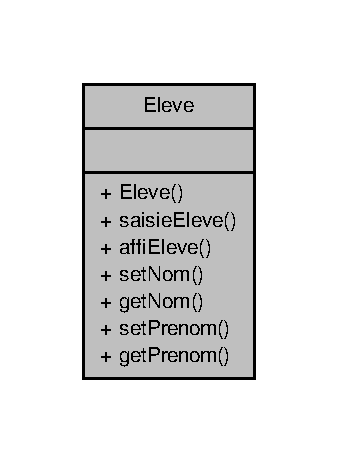
\includegraphics[width=162pt]{class_eleve__coll__graph}
\end{center}
\end{figure}
\subsection*{Fonctions membres publiques}
\begin{DoxyCompactItemize}
\item 
\hyperlink{class_eleve_ac17e7d7daabe4fb88306fe3fe003bdc7}{Eleve} ()
\item 
void \hyperlink{class_eleve_a58dfffa4ec2e1098cca621aca1bc8b01}{saisie\-Eleve} ()
\begin{DoxyCompactList}\small\item\em saisie d'un élève $\ast$\-Permet à l'utilisateur de saisir les informations d'un élève \end{DoxyCompactList}\item 
void \hyperlink{class_eleve_a4c52b8dc64acde0c0f6616773d361e27}{affi\-Eleve} ()
\begin{DoxyCompactList}\small\item\em affiche élève $\ast$\-Permet d'afficher les informations d'un élève \end{DoxyCompactList}\item 
void \hyperlink{class_eleve_a9ae9b9ab1bdad31358aaabfe782ee917}{set\-Nom} (string new\-\_\-var)
\begin{DoxyCompactList}\small\item\em $\ast$\-Permet de donner un nom à un élève \end{DoxyCompactList}\item 
string \hyperlink{class_eleve_abf63239397983c10c4dfea36839aa522}{get\-Nom} ()
\begin{DoxyCompactList}\small\item\em $\ast$\-Permet de retourner le nom de l'élève \end{DoxyCompactList}\item 
void \hyperlink{class_eleve_a204474920420c637c2db34676fa5b6f1}{set\-Prenom} (string new\-\_\-var)
\begin{DoxyCompactList}\small\item\em $\ast$\-Permet de donner un prénom à un élève \end{DoxyCompactList}\item 
string \hyperlink{class_eleve_a306ededf39fac45344ceb81f4591d96f}{get\-Prenom} ()
\end{DoxyCompactItemize}


\subsection{Description détaillée}
class \hyperlink{class_eleve}{Eleve} 

\subsection{Documentation des constructeurs et destructeur}
\hypertarget{class_eleve_ac17e7d7daabe4fb88306fe3fe003bdc7}{\index{Eleve@{Eleve}!Eleve@{Eleve}}
\index{Eleve@{Eleve}!Eleve@{Eleve}}
\subsubsection[{Eleve}]{\setlength{\rightskip}{0pt plus 5cm}Eleve\-::\-Eleve (
\begin{DoxyParamCaption}
{}
\end{DoxyParamCaption}
)}}\label{class_eleve_ac17e7d7daabe4fb88306fe3fe003bdc7}
Empty Constructor 

\subsection{Documentation des fonctions membres}
\hypertarget{class_eleve_a4c52b8dc64acde0c0f6616773d361e27}{\index{Eleve@{Eleve}!affi\-Eleve@{affi\-Eleve}}
\index{affi\-Eleve@{affi\-Eleve}!Eleve@{Eleve}}
\subsubsection[{affi\-Eleve}]{\setlength{\rightskip}{0pt plus 5cm}void Eleve\-::affi\-Eleve (
\begin{DoxyParamCaption}
{}
\end{DoxyParamCaption}
)}}\label{class_eleve_a4c52b8dc64acde0c0f6616773d361e27}


affiche élève $\ast$\-Permet d'afficher les informations d'un élève 



Voici le graphe d'appel pour cette fonction \-:
\nopagebreak
\begin{figure}[H]
\begin{center}
\leavevmode
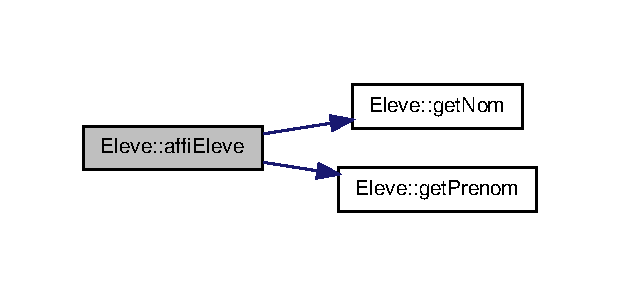
\includegraphics[width=298pt]{class_eleve_a4c52b8dc64acde0c0f6616773d361e27_cgraph}
\end{center}
\end{figure}


\hypertarget{class_eleve_abf63239397983c10c4dfea36839aa522}{\index{Eleve@{Eleve}!get\-Nom@{get\-Nom}}
\index{get\-Nom@{get\-Nom}!Eleve@{Eleve}}
\subsubsection[{get\-Nom}]{\setlength{\rightskip}{0pt plus 5cm}string Eleve\-::get\-Nom (
\begin{DoxyParamCaption}
{}
\end{DoxyParamCaption}
)}}\label{class_eleve_abf63239397983c10c4dfea36839aa522}


$\ast$\-Permet de retourner le nom de l'élève 

Get the value of nom \begin{DoxyReturn}{Renvoie}
the value of nom 
\end{DoxyReturn}


Voici le graphe des appelants de cette fonction \-:
\nopagebreak
\begin{figure}[H]
\begin{center}
\leavevmode
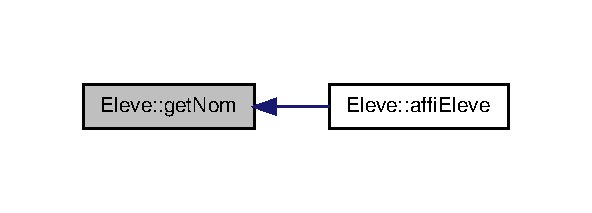
\includegraphics[width=284pt]{class_eleve_abf63239397983c10c4dfea36839aa522_icgraph}
\end{center}
\end{figure}


\hypertarget{class_eleve_a306ededf39fac45344ceb81f4591d96f}{\index{Eleve@{Eleve}!get\-Prenom@{get\-Prenom}}
\index{get\-Prenom@{get\-Prenom}!Eleve@{Eleve}}
\subsubsection[{get\-Prenom}]{\setlength{\rightskip}{0pt plus 5cm}string Eleve\-::get\-Prenom (
\begin{DoxyParamCaption}
{}
\end{DoxyParamCaption}
)}}\label{class_eleve_a306ededf39fac45344ceb81f4591d96f}
$\ast$\-Permet de retourner le prénom de l'élève

Get the value of prenom \begin{DoxyReturn}{Renvoie}
the value of prenom 
\end{DoxyReturn}


Voici le graphe des appelants de cette fonction \-:
\nopagebreak
\begin{figure}[H]
\begin{center}
\leavevmode
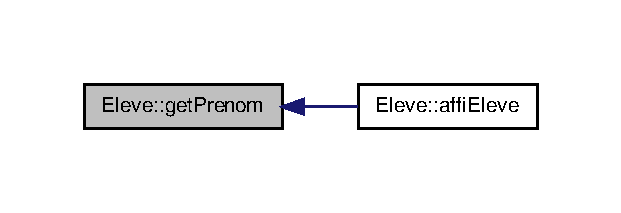
\includegraphics[width=298pt]{class_eleve_a306ededf39fac45344ceb81f4591d96f_icgraph}
\end{center}
\end{figure}


\hypertarget{class_eleve_a58dfffa4ec2e1098cca621aca1bc8b01}{\index{Eleve@{Eleve}!saisie\-Eleve@{saisie\-Eleve}}
\index{saisie\-Eleve@{saisie\-Eleve}!Eleve@{Eleve}}
\subsubsection[{saisie\-Eleve}]{\setlength{\rightskip}{0pt plus 5cm}void Eleve\-::saisie\-Eleve (
\begin{DoxyParamCaption}
{}
\end{DoxyParamCaption}
)}}\label{class_eleve_a58dfffa4ec2e1098cca621aca1bc8b01}


saisie d'un élève $\ast$\-Permet à l'utilisateur de saisir les informations d'un élève 



Voici le graphe d'appel pour cette fonction \-:
\nopagebreak
\begin{figure}[H]
\begin{center}
\leavevmode
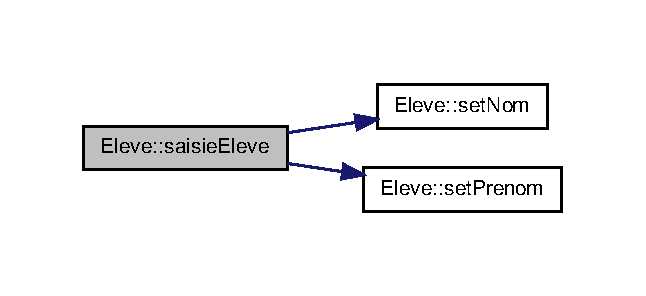
\includegraphics[width=310pt]{class_eleve_a58dfffa4ec2e1098cca621aca1bc8b01_cgraph}
\end{center}
\end{figure}




Voici le graphe des appelants de cette fonction \-:
\nopagebreak
\begin{figure}[H]
\begin{center}
\leavevmode
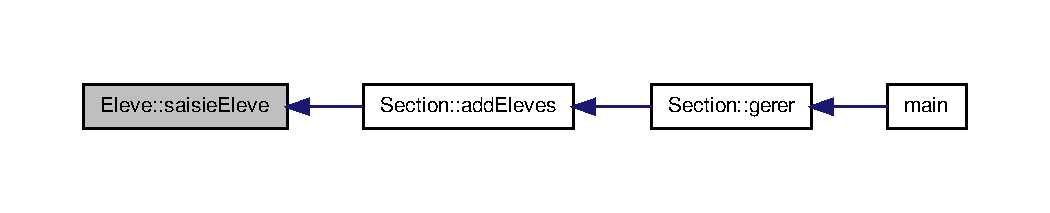
\includegraphics[width=350pt]{class_eleve_a58dfffa4ec2e1098cca621aca1bc8b01_icgraph}
\end{center}
\end{figure}


\hypertarget{class_eleve_a9ae9b9ab1bdad31358aaabfe782ee917}{\index{Eleve@{Eleve}!set\-Nom@{set\-Nom}}
\index{set\-Nom@{set\-Nom}!Eleve@{Eleve}}
\subsubsection[{set\-Nom}]{\setlength{\rightskip}{0pt plus 5cm}void Eleve\-::set\-Nom (
\begin{DoxyParamCaption}
\item[{string}]{new\-\_\-var}
\end{DoxyParamCaption}
)}}\label{class_eleve_a9ae9b9ab1bdad31358aaabfe782ee917}


$\ast$\-Permet de donner un nom à un élève 

Set the value of nom 
\begin{DoxyParams}{Paramètres}
{\em new\-\_\-var} & the new value of nom \\
\hline
\end{DoxyParams}


Voici le graphe des appelants de cette fonction \-:
\nopagebreak
\begin{figure}[H]
\begin{center}
\leavevmode
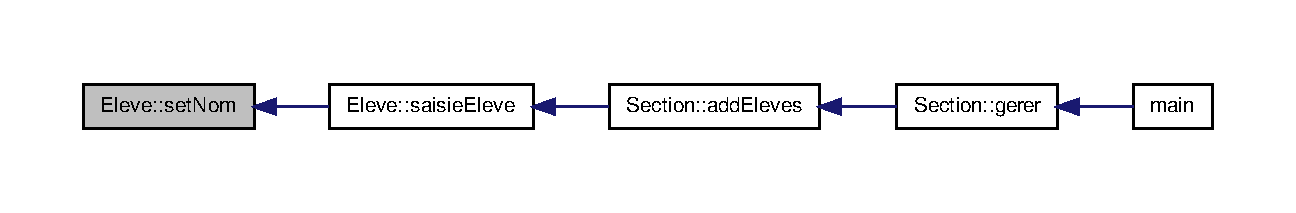
\includegraphics[width=350pt]{class_eleve_a9ae9b9ab1bdad31358aaabfe782ee917_icgraph}
\end{center}
\end{figure}


\hypertarget{class_eleve_a204474920420c637c2db34676fa5b6f1}{\index{Eleve@{Eleve}!set\-Prenom@{set\-Prenom}}
\index{set\-Prenom@{set\-Prenom}!Eleve@{Eleve}}
\subsubsection[{set\-Prenom}]{\setlength{\rightskip}{0pt plus 5cm}void Eleve\-::set\-Prenom (
\begin{DoxyParamCaption}
\item[{string}]{new\-\_\-var}
\end{DoxyParamCaption}
)}}\label{class_eleve_a204474920420c637c2db34676fa5b6f1}


$\ast$\-Permet de donner un prénom à un élève 

Set the value of prenom 
\begin{DoxyParams}{Paramètres}
{\em new\-\_\-var} & the new value of prenom \\
\hline
\end{DoxyParams}


Voici le graphe des appelants de cette fonction \-:
\nopagebreak
\begin{figure}[H]
\begin{center}
\leavevmode
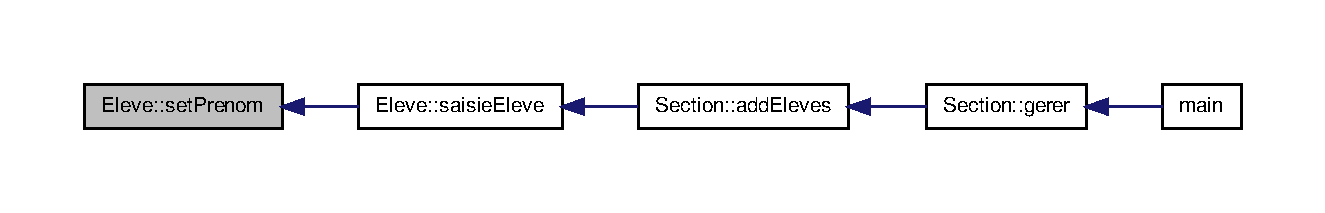
\includegraphics[width=350pt]{class_eleve_a204474920420c637c2db34676fa5b6f1_icgraph}
\end{center}
\end{figure}




La documentation de cette classe a été générée à partir des fichiers suivants \-:\begin{DoxyCompactItemize}
\item 
\hyperlink{eleve_8h}{eleve.\-h}\item 
\hyperlink{eleve_8cpp}{eleve.\-cpp}\end{DoxyCompactItemize}

\hypertarget{class_evaluation}{\section{Référence de la classe Evaluation}
\label{class_evaluation}\index{Evaluation@{Evaluation}}
}


{\ttfamily \#include $<$Evaluation.\-h$>$}



Graphe de collaboration de Evaluation\-:
\nopagebreak
\begin{figure}[H]
\begin{center}
\leavevmode
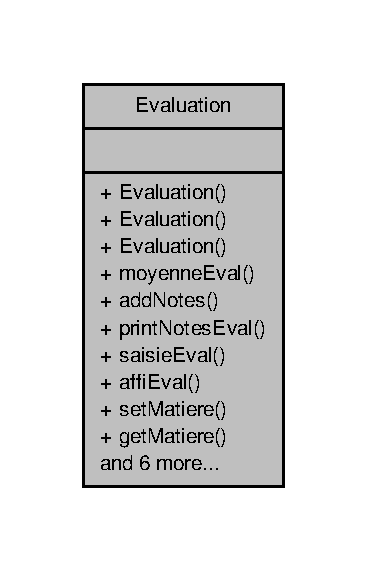
\includegraphics[width=176pt]{class_evaluation__coll__graph}
\end{center}
\end{figure}
\subsection*{Fonctions membres publiques}
\begin{DoxyCompactItemize}
\item 
\hyperlink{class_evaluation_af7b959b9a214ba6bd0ecc65324d9fe12}{Evaluation} ()
\begin{DoxyCompactList}\small\item\em constructeur vide $\ast$\-Permet de créer une évaluation \end{DoxyCompactList}\item 
\hyperlink{class_evaluation_ac314d2138cbce24223f66ce52d3fab51}{Evaluation} (int l\-Id, int le\-Coeff, string la\-Date)
\begin{DoxyCompactList}\small\item\em constructeur id+coeff+date $\ast$\-Permet d'instancier une évaluation en lui donnant un id, un coeff et une date \end{DoxyCompactList}\item 
\hyperlink{class_evaluation_a9d8bd540b9c6bf9f0f29b66c33384785}{Evaluation} (int l\-Id, int le\-Coeff, string la\-Date, \hyperlink{class_matiere}{Matiere} $\ast$la\-Matiere)
\begin{DoxyCompactList}\small\item\em constructeur id+coeff+date+matiere $\ast$\-Permet d'instancier une évaluation en lui donnant un id, un coeff, une date et une matière \end{DoxyCompactList}\item 
double \hyperlink{class_evaluation_ab51c8ccf98e731b48c7d12586b0cdfab}{moyenne\-Eval} ()
\begin{DoxyCompactList}\small\item\em moyenne évaluation $\ast$\-Permet de calculer la moyenne d'une évaluation \end{DoxyCompactList}\item 
void \hyperlink{class_evaluation_ac1b064b52d0a8527d046130a0c352743}{add\-Notes} ()
\begin{DoxyCompactList}\small\item\em ajouter notes $\ast$\-Permet d'ajouter des notes dans le vecteur notes d'une évaluation \end{DoxyCompactList}\item 
void \hyperlink{class_evaluation_aa9a018cc4136e5aba6a73dcfaaf88d8a}{print\-Notes\-Eval} ()
\begin{DoxyCompactList}\small\item\em afficher notes de l'évaluation $\ast$\-Permet d'affiche toutes les notes d'une évaluation précise \end{DoxyCompactList}\item 
void \hyperlink{class_evaluation_a7bca2f24b3cd48bc41220c4ad127a10f}{saisie\-Eval} (\hyperlink{class_matiere}{Matiere} $\ast$new\-Mat)
\begin{DoxyCompactList}\small\item\em saisie évaluation $\ast$\-Permet à l'utilisateur de saisir une évaluation \end{DoxyCompactList}\item 
void \hyperlink{class_evaluation_a3cb34d3397cceeff0e3ce51badc7cf83}{affi\-Eval} ()
\begin{DoxyCompactList}\small\item\em afficher évaluation $\ast$\-Permet d'afficher le descriptif d'une évaluation \end{DoxyCompactList}\item 
void \hyperlink{class_evaluation_a5093357701d653d150471933d86c905c}{set\-Matiere} (\hyperlink{class_matiere}{Matiere} $\ast$new\-\_\-var)
\begin{DoxyCompactList}\small\item\em $\ast$\-Permet de donner une matiere à l'évaluation \end{DoxyCompactList}\item 
\hyperlink{class_matiere}{Matiere} $\ast$ \hyperlink{class_evaluation_ab74c781aaf29c0c43ac5c04d9ff74065}{get\-Matiere} ()
\begin{DoxyCompactList}\small\item\em $\ast$permet de retourner la matière d'une évaluation \end{DoxyCompactList}\item 
void \hyperlink{class_evaluation_a9da8c5e1c7c580dda5d2e5509771dd5a}{set\-Id} (int new\-\_\-var)
\begin{DoxyCompactList}\small\item\em $\ast$\-Permet de donner un id à l'évaluation \end{DoxyCompactList}\item 
int \hyperlink{class_evaluation_a7321d761cd51da691fb1712e878852f6}{get\-Id} ()
\begin{DoxyCompactList}\small\item\em $\ast$\-Permet de retourner l'id de l'évaluation \end{DoxyCompactList}\item 
void \hyperlink{class_evaluation_a71abf2df2a50639d207b94d8cacd7206}{set\-Coeff} (int new\-\_\-var)
\begin{DoxyCompactList}\small\item\em $\ast$\-Permet de donenr un coeff à l'évaluation \end{DoxyCompactList}\item 
int \hyperlink{class_evaluation_af4c2323e59d3344226d1e760f74f00c2}{get\-Coeff} ()
\begin{DoxyCompactList}\small\item\em $\ast$\-Permet de retourner un coeff de l'évaluation \end{DoxyCompactList}\item 
void \hyperlink{class_evaluation_a6a84b62167fab19b8d74e8f225c3a622}{set\-Date} (string la\-Date)
\begin{DoxyCompactList}\small\item\em $\ast$\-Permet de donner une date à l'évaluation \end{DoxyCompactList}\item 
string \hyperlink{class_evaluation_a737df75c5f979ec212554209f9224a6e}{get\-Date} ()
\begin{DoxyCompactList}\small\item\em $\ast$\-Permet de retourner la date de l'évaluation \end{DoxyCompactList}\end{DoxyCompactItemize}


\subsection{Description détaillée}
class \hyperlink{class_evaluation}{Evaluation} 

\subsection{Documentation des constructeurs et destructeur}
\hypertarget{class_evaluation_af7b959b9a214ba6bd0ecc65324d9fe12}{\index{Evaluation@{Evaluation}!Evaluation@{Evaluation}}
\index{Evaluation@{Evaluation}!Evaluation@{Evaluation}}
\subsubsection[{Evaluation}]{\setlength{\rightskip}{0pt plus 5cm}Evaluation\-::\-Evaluation (
\begin{DoxyParamCaption}
{}
\end{DoxyParamCaption}
)}}\label{class_evaluation_af7b959b9a214ba6bd0ecc65324d9fe12}


constructeur vide $\ast$\-Permet de créer une évaluation 

\hypertarget{class_evaluation_ac314d2138cbce24223f66ce52d3fab51}{\index{Evaluation@{Evaluation}!Evaluation@{Evaluation}}
\index{Evaluation@{Evaluation}!Evaluation@{Evaluation}}
\subsubsection[{Evaluation}]{\setlength{\rightskip}{0pt plus 5cm}Evaluation\-::\-Evaluation (
\begin{DoxyParamCaption}
\item[{int}]{l\-Id, }
\item[{int}]{le\-Coeff, }
\item[{string}]{la\-Date}
\end{DoxyParamCaption}
)}}\label{class_evaluation_ac314d2138cbce24223f66ce52d3fab51}


constructeur id+coeff+date $\ast$\-Permet d'instancier une évaluation en lui donnant un id, un coeff et une date 


\begin{DoxyParams}{Paramètres}
{\em l'id} & puis le coeff et enfin la date de l'évaluation que l'on veut créer \\
\hline
\end{DoxyParams}
\hypertarget{class_evaluation_a9d8bd540b9c6bf9f0f29b66c33384785}{\index{Evaluation@{Evaluation}!Evaluation@{Evaluation}}
\index{Evaluation@{Evaluation}!Evaluation@{Evaluation}}
\subsubsection[{Evaluation}]{\setlength{\rightskip}{0pt plus 5cm}Evaluation\-::\-Evaluation (
\begin{DoxyParamCaption}
\item[{int}]{l\-Id, }
\item[{int}]{le\-Coeff, }
\item[{string}]{la\-Date, }
\item[{{\bf Matiere} $\ast$}]{la\-Matiere}
\end{DoxyParamCaption}
)}}\label{class_evaluation_a9d8bd540b9c6bf9f0f29b66c33384785}


constructeur id+coeff+date+matiere $\ast$\-Permet d'instancier une évaluation en lui donnant un id, un coeff, une date et une matière 


\begin{DoxyParams}{Paramètres}
{\em l'id} & puis le coeff puis la date et enfin une matière de l'évaluation que l'on veut créer \\
\hline
\end{DoxyParams}


\subsection{Documentation des fonctions membres}
\hypertarget{class_evaluation_ac1b064b52d0a8527d046130a0c352743}{\index{Evaluation@{Evaluation}!add\-Notes@{add\-Notes}}
\index{add\-Notes@{add\-Notes}!Evaluation@{Evaluation}}
\subsubsection[{add\-Notes}]{\setlength{\rightskip}{0pt plus 5cm}void Evaluation\-::add\-Notes (
\begin{DoxyParamCaption}
{}
\end{DoxyParamCaption}
)}}\label{class_evaluation_ac1b064b52d0a8527d046130a0c352743}


ajouter notes $\ast$\-Permet d'ajouter des notes dans le vecteur notes d'une évaluation 



Voici le graphe d'appel pour cette fonction \-:
\nopagebreak
\begin{figure}[H]
\begin{center}
\leavevmode
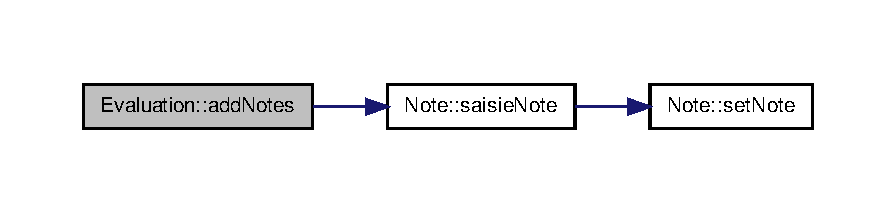
\includegraphics[width=350pt]{class_evaluation_ac1b064b52d0a8527d046130a0c352743_cgraph}
\end{center}
\end{figure}


\hypertarget{class_evaluation_a3cb34d3397cceeff0e3ce51badc7cf83}{\index{Evaluation@{Evaluation}!affi\-Eval@{affi\-Eval}}
\index{affi\-Eval@{affi\-Eval}!Evaluation@{Evaluation}}
\subsubsection[{affi\-Eval}]{\setlength{\rightskip}{0pt plus 5cm}void Evaluation\-::affi\-Eval (
\begin{DoxyParamCaption}
{}
\end{DoxyParamCaption}
)}}\label{class_evaluation_a3cb34d3397cceeff0e3ce51badc7cf83}


afficher évaluation $\ast$\-Permet d'afficher le descriptif d'une évaluation 



Voici le graphe d'appel pour cette fonction \-:
\nopagebreak
\begin{figure}[H]
\begin{center}
\leavevmode
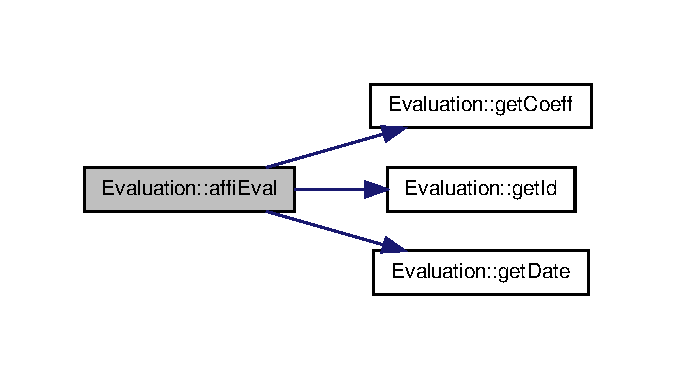
\includegraphics[width=324pt]{class_evaluation_a3cb34d3397cceeff0e3ce51badc7cf83_cgraph}
\end{center}
\end{figure}


\hypertarget{class_evaluation_af4c2323e59d3344226d1e760f74f00c2}{\index{Evaluation@{Evaluation}!get\-Coeff@{get\-Coeff}}
\index{get\-Coeff@{get\-Coeff}!Evaluation@{Evaluation}}
\subsubsection[{get\-Coeff}]{\setlength{\rightskip}{0pt plus 5cm}int Evaluation\-::get\-Coeff (
\begin{DoxyParamCaption}
{}
\end{DoxyParamCaption}
)}}\label{class_evaluation_af4c2323e59d3344226d1e760f74f00c2}


$\ast$\-Permet de retourner un coeff de l'évaluation 

Get the value of coeff \begin{DoxyReturn}{Renvoie}
the value of coeff 
\end{DoxyReturn}


Voici le graphe des appelants de cette fonction \-:
\nopagebreak
\begin{figure}[H]
\begin{center}
\leavevmode
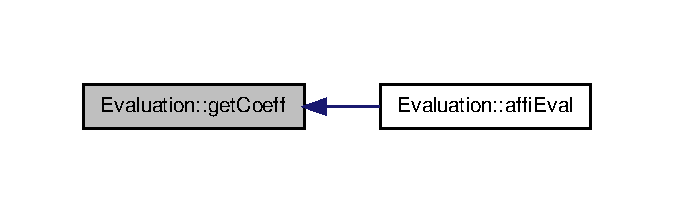
\includegraphics[width=324pt]{class_evaluation_af4c2323e59d3344226d1e760f74f00c2_icgraph}
\end{center}
\end{figure}


\hypertarget{class_evaluation_a737df75c5f979ec212554209f9224a6e}{\index{Evaluation@{Evaluation}!get\-Date@{get\-Date}}
\index{get\-Date@{get\-Date}!Evaluation@{Evaluation}}
\subsubsection[{get\-Date}]{\setlength{\rightskip}{0pt plus 5cm}string Evaluation\-::get\-Date (
\begin{DoxyParamCaption}
{}
\end{DoxyParamCaption}
)}}\label{class_evaluation_a737df75c5f979ec212554209f9224a6e}


$\ast$\-Permet de retourner la date de l'évaluation 



Voici le graphe des appelants de cette fonction \-:
\nopagebreak
\begin{figure}[H]
\begin{center}
\leavevmode
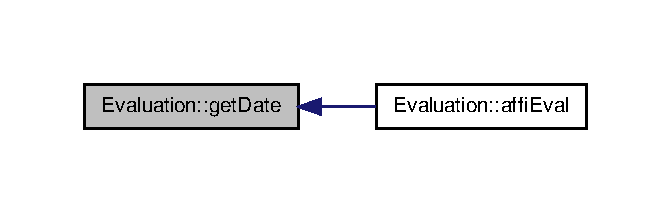
\includegraphics[width=322pt]{class_evaluation_a737df75c5f979ec212554209f9224a6e_icgraph}
\end{center}
\end{figure}


\hypertarget{class_evaluation_a7321d761cd51da691fb1712e878852f6}{\index{Evaluation@{Evaluation}!get\-Id@{get\-Id}}
\index{get\-Id@{get\-Id}!Evaluation@{Evaluation}}
\subsubsection[{get\-Id}]{\setlength{\rightskip}{0pt plus 5cm}int Evaluation\-::get\-Id (
\begin{DoxyParamCaption}
{}
\end{DoxyParamCaption}
)}}\label{class_evaluation_a7321d761cd51da691fb1712e878852f6}


$\ast$\-Permet de retourner l'id de l'évaluation 

Get the value of id \begin{DoxyReturn}{Renvoie}
the value of id 
\end{DoxyReturn}


Voici le graphe des appelants de cette fonction \-:
\nopagebreak
\begin{figure}[H]
\begin{center}
\leavevmode
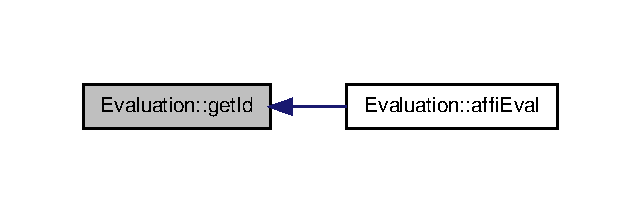
\includegraphics[width=308pt]{class_evaluation_a7321d761cd51da691fb1712e878852f6_icgraph}
\end{center}
\end{figure}


\hypertarget{class_evaluation_ab74c781aaf29c0c43ac5c04d9ff74065}{\index{Evaluation@{Evaluation}!get\-Matiere@{get\-Matiere}}
\index{get\-Matiere@{get\-Matiere}!Evaluation@{Evaluation}}
\subsubsection[{get\-Matiere}]{\setlength{\rightskip}{0pt plus 5cm}{\bf Matiere} $\ast$ Evaluation\-::get\-Matiere (
\begin{DoxyParamCaption}
{}
\end{DoxyParamCaption}
)}}\label{class_evaluation_ab74c781aaf29c0c43ac5c04d9ff74065}


$\ast$permet de retourner la matière d'une évaluation 

Get the value of matiere \begin{DoxyReturn}{Renvoie}
the value of matiere 
\end{DoxyReturn}
\hypertarget{class_evaluation_ab51c8ccf98e731b48c7d12586b0cdfab}{\index{Evaluation@{Evaluation}!moyenne\-Eval@{moyenne\-Eval}}
\index{moyenne\-Eval@{moyenne\-Eval}!Evaluation@{Evaluation}}
\subsubsection[{moyenne\-Eval}]{\setlength{\rightskip}{0pt plus 5cm}double Evaluation\-::moyenne\-Eval (
\begin{DoxyParamCaption}
{}
\end{DoxyParamCaption}
)}}\label{class_evaluation_ab51c8ccf98e731b48c7d12586b0cdfab}


moyenne évaluation $\ast$\-Permet de calculer la moyenne d'une évaluation 

\hypertarget{class_evaluation_aa9a018cc4136e5aba6a73dcfaaf88d8a}{\index{Evaluation@{Evaluation}!print\-Notes\-Eval@{print\-Notes\-Eval}}
\index{print\-Notes\-Eval@{print\-Notes\-Eval}!Evaluation@{Evaluation}}
\subsubsection[{print\-Notes\-Eval}]{\setlength{\rightskip}{0pt plus 5cm}void Evaluation\-::print\-Notes\-Eval (
\begin{DoxyParamCaption}
{}
\end{DoxyParamCaption}
)}}\label{class_evaluation_aa9a018cc4136e5aba6a73dcfaaf88d8a}


afficher notes de l'évaluation $\ast$\-Permet d'affiche toutes les notes d'une évaluation précise 

\hypertarget{class_evaluation_a7bca2f24b3cd48bc41220c4ad127a10f}{\index{Evaluation@{Evaluation}!saisie\-Eval@{saisie\-Eval}}
\index{saisie\-Eval@{saisie\-Eval}!Evaluation@{Evaluation}}
\subsubsection[{saisie\-Eval}]{\setlength{\rightskip}{0pt plus 5cm}void Evaluation\-::saisie\-Eval (
\begin{DoxyParamCaption}
\item[{{\bf Matiere} $\ast$}]{new\-Mat}
\end{DoxyParamCaption}
)}}\label{class_evaluation_a7bca2f24b3cd48bc41220c4ad127a10f}


saisie évaluation $\ast$\-Permet à l'utilisateur de saisir une évaluation 


\begin{DoxyParams}{Paramètres}
{\em une} & matière \\
\hline
\end{DoxyParams}


Voici le graphe d'appel pour cette fonction \-:
\nopagebreak
\begin{figure}[H]
\begin{center}
\leavevmode
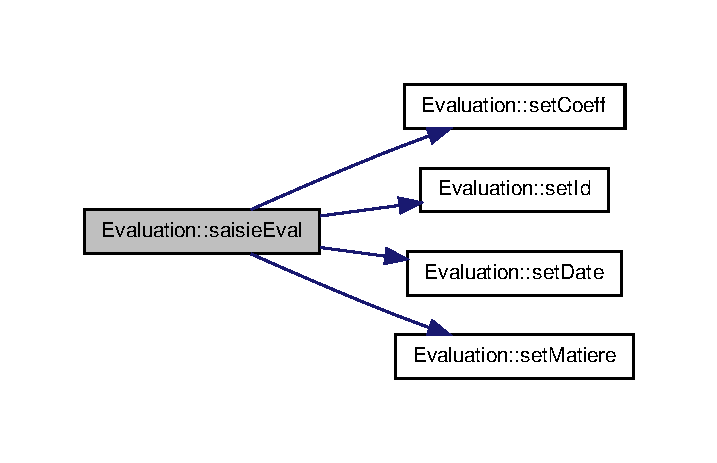
\includegraphics[width=344pt]{class_evaluation_a7bca2f24b3cd48bc41220c4ad127a10f_cgraph}
\end{center}
\end{figure}




Voici le graphe des appelants de cette fonction \-:
\nopagebreak
\begin{figure}[H]
\begin{center}
\leavevmode
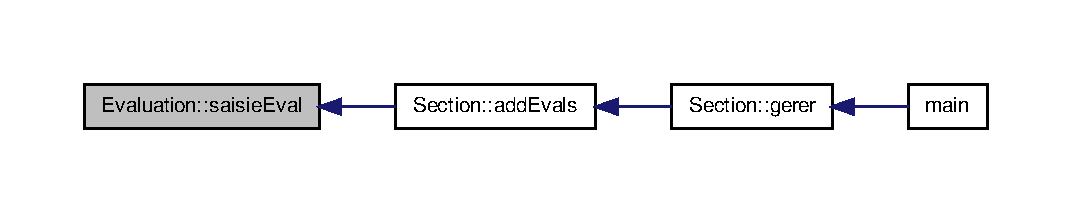
\includegraphics[width=350pt]{class_evaluation_a7bca2f24b3cd48bc41220c4ad127a10f_icgraph}
\end{center}
\end{figure}


\hypertarget{class_evaluation_a71abf2df2a50639d207b94d8cacd7206}{\index{Evaluation@{Evaluation}!set\-Coeff@{set\-Coeff}}
\index{set\-Coeff@{set\-Coeff}!Evaluation@{Evaluation}}
\subsubsection[{set\-Coeff}]{\setlength{\rightskip}{0pt plus 5cm}void Evaluation\-::set\-Coeff (
\begin{DoxyParamCaption}
\item[{int}]{new\-\_\-var}
\end{DoxyParamCaption}
)}}\label{class_evaluation_a71abf2df2a50639d207b94d8cacd7206}


$\ast$\-Permet de donenr un coeff à l'évaluation 

Set the value of coeff 
\begin{DoxyParams}{Paramètres}
{\em new\-\_\-var} & the new value of coeff \\
\hline
\end{DoxyParams}


Voici le graphe des appelants de cette fonction \-:
\nopagebreak
\begin{figure}[H]
\begin{center}
\leavevmode
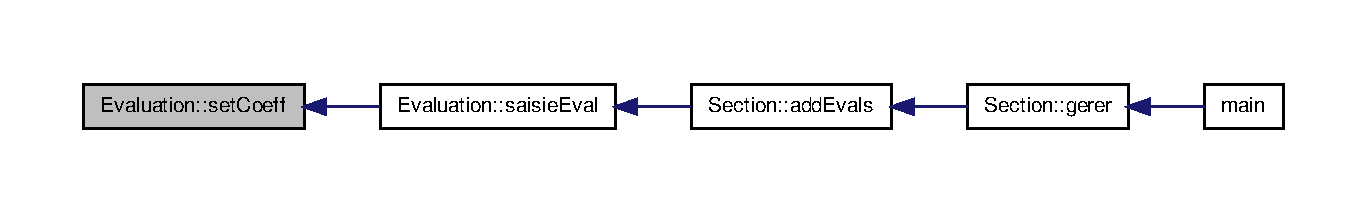
\includegraphics[width=350pt]{class_evaluation_a71abf2df2a50639d207b94d8cacd7206_icgraph}
\end{center}
\end{figure}


\hypertarget{class_evaluation_a6a84b62167fab19b8d74e8f225c3a622}{\index{Evaluation@{Evaluation}!set\-Date@{set\-Date}}
\index{set\-Date@{set\-Date}!Evaluation@{Evaluation}}
\subsubsection[{set\-Date}]{\setlength{\rightskip}{0pt plus 5cm}void Evaluation\-::set\-Date (
\begin{DoxyParamCaption}
\item[{string}]{la\-Date}
\end{DoxyParamCaption}
)}}\label{class_evaluation_a6a84b62167fab19b8d74e8f225c3a622}


$\ast$\-Permet de donner une date à l'évaluation 



Voici le graphe des appelants de cette fonction \-:
\nopagebreak
\begin{figure}[H]
\begin{center}
\leavevmode
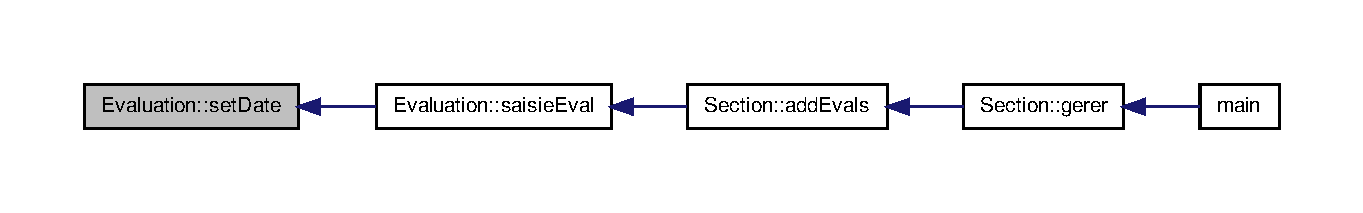
\includegraphics[width=350pt]{class_evaluation_a6a84b62167fab19b8d74e8f225c3a622_icgraph}
\end{center}
\end{figure}


\hypertarget{class_evaluation_a9da8c5e1c7c580dda5d2e5509771dd5a}{\index{Evaluation@{Evaluation}!set\-Id@{set\-Id}}
\index{set\-Id@{set\-Id}!Evaluation@{Evaluation}}
\subsubsection[{set\-Id}]{\setlength{\rightskip}{0pt plus 5cm}void Evaluation\-::set\-Id (
\begin{DoxyParamCaption}
\item[{int}]{new\-\_\-var}
\end{DoxyParamCaption}
)}}\label{class_evaluation_a9da8c5e1c7c580dda5d2e5509771dd5a}


$\ast$\-Permet de donner un id à l'évaluation 

Set the value of id 
\begin{DoxyParams}{Paramètres}
{\em new\-\_\-var} & the new value of id \\
\hline
\end{DoxyParams}


Voici le graphe des appelants de cette fonction \-:
\nopagebreak
\begin{figure}[H]
\begin{center}
\leavevmode
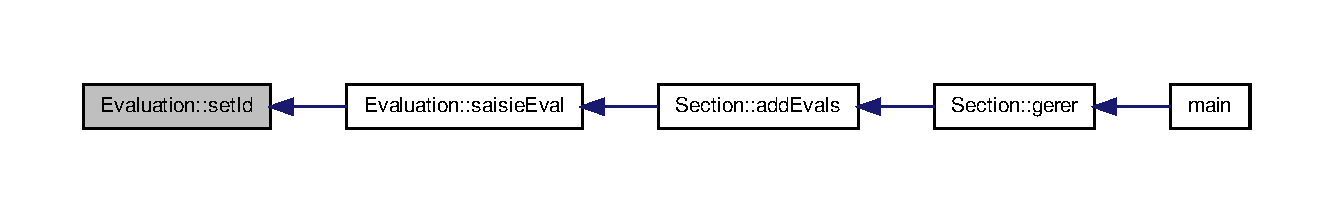
\includegraphics[width=350pt]{class_evaluation_a9da8c5e1c7c580dda5d2e5509771dd5a_icgraph}
\end{center}
\end{figure}


\hypertarget{class_evaluation_a5093357701d653d150471933d86c905c}{\index{Evaluation@{Evaluation}!set\-Matiere@{set\-Matiere}}
\index{set\-Matiere@{set\-Matiere}!Evaluation@{Evaluation}}
\subsubsection[{set\-Matiere}]{\setlength{\rightskip}{0pt plus 5cm}void Evaluation\-::set\-Matiere (
\begin{DoxyParamCaption}
\item[{{\bf Matiere} $\ast$}]{new\-\_\-var}
\end{DoxyParamCaption}
)}}\label{class_evaluation_a5093357701d653d150471933d86c905c}


$\ast$\-Permet de donner une matiere à l'évaluation 

Set the value of matiere 
\begin{DoxyParams}{Paramètres}
{\em new\-\_\-var} & the new value of matiere \\
\hline
\end{DoxyParams}


Voici le graphe des appelants de cette fonction \-:
\nopagebreak
\begin{figure}[H]
\begin{center}
\leavevmode
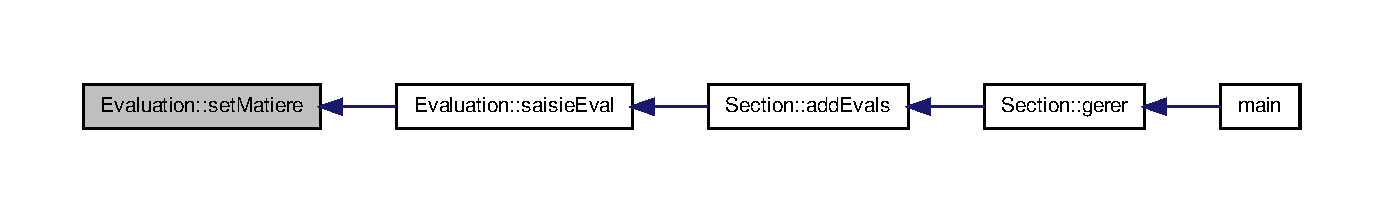
\includegraphics[width=350pt]{class_evaluation_a5093357701d653d150471933d86c905c_icgraph}
\end{center}
\end{figure}




La documentation de cette classe a été générée à partir des fichiers suivants \-:\begin{DoxyCompactItemize}
\item 
\hyperlink{_evaluation_8h}{Evaluation.\-h}\item 
\hyperlink{_evaluation_8cpp}{Evaluation.\-cpp}\end{DoxyCompactItemize}

\hypertarget{class_matiere}{\section{Référence de la classe Matiere}
\label{class_matiere}\index{Matiere@{Matiere}}
}


{\ttfamily \#include $<$Matiere.\-h$>$}



Graphe de collaboration de Matiere\-:
\nopagebreak
\begin{figure}[H]
\begin{center}
\leavevmode
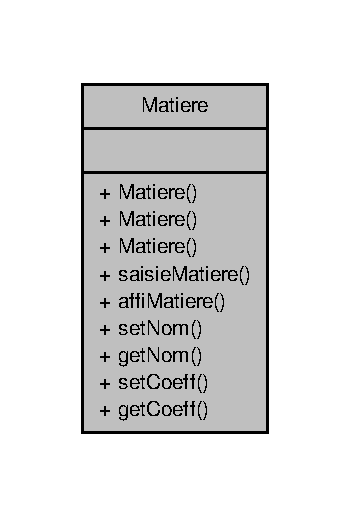
\includegraphics[width=168pt]{class_matiere__coll__graph}
\end{center}
\end{figure}
\subsection*{Fonctions membres publiques}
\begin{DoxyCompactItemize}
\item 
\hyperlink{class_matiere_a0d9dbc35cd0221225366e2ba189c4b42}{Matiere} ()
\item 
\hyperlink{class_matiere_a272664e39fe50d84a258ef9ec798f096}{Matiere} (string le\-Nom)
\begin{DoxyCompactList}\small\item\em constructeur nom $\ast$\-Permet de créer une matière en initialisasnt seulement le nom \end{DoxyCompactList}\item 
\hyperlink{class_matiere_a38b701f4d07921ba6331de18be20ab77}{Matiere} (string le\-Nom, int le\-Coeff)
\begin{DoxyCompactList}\small\item\em constructeur nom + coeff $\ast$\-Permet de créer une matère en initialisant le nom et le coeff \end{DoxyCompactList}\item 
void \hyperlink{class_matiere_ac84968e1561a24e5118468edc2750f4f}{saisie\-Matiere} ()
\begin{DoxyCompactList}\small\item\em saisir une Matière $\ast$\-Permet à l'utilisateur de saisir toutes les informations de la matière \end{DoxyCompactList}\item 
void \hyperlink{class_matiere_a40ce0a7003b3d771bbcb2c745a20ad1a}{affi\-Matiere} ()
\begin{DoxyCompactList}\small\item\em afficher une matière $\ast$\-Permet d'afficher les informations d'une matière \end{DoxyCompactList}\item 
void \hyperlink{class_matiere_ae0d9312f6cbddf446614ffa00d1750ae}{set\-Nom} (string new\-\_\-var)
\begin{DoxyCompactList}\small\item\em $\ast$permet de donner un nom à une matière \end{DoxyCompactList}\item 
string \hyperlink{class_matiere_a103abd445b1bc378e0e3687875f4fcff}{get\-Nom} ()
\begin{DoxyCompactList}\small\item\em $\ast$\-Permet de retourner le nom d'une matière \end{DoxyCompactList}\item 
void \hyperlink{class_matiere_aabf35dcc826eedca91490b8985d67da7}{set\-Coeff} (int new\-\_\-var)
\begin{DoxyCompactList}\small\item\em $\ast$\-Permet de donner un coeff à une matière \end{DoxyCompactList}\item 
int \hyperlink{class_matiere_a3e50f81ac7893dbd989c9d06ff9af763}{get\-Coeff} ()
\begin{DoxyCompactList}\small\item\em $\ast$\-Permet de retourner le coeff de la matière \end{DoxyCompactList}\end{DoxyCompactItemize}


\subsection{Description détaillée}
class \hyperlink{class_matiere}{Matiere} Une matiere est une des parties enseigner. 

\subsection{Documentation des constructeurs et destructeur}
\hypertarget{class_matiere_a0d9dbc35cd0221225366e2ba189c4b42}{\index{Matiere@{Matiere}!Matiere@{Matiere}}
\index{Matiere@{Matiere}!Matiere@{Matiere}}
\subsubsection[{Matiere}]{\setlength{\rightskip}{0pt plus 5cm}Matiere\-::\-Matiere (
\begin{DoxyParamCaption}
{}
\end{DoxyParamCaption}
)}}\label{class_matiere_a0d9dbc35cd0221225366e2ba189c4b42}
$\ast$\-Constructeur \hypertarget{class_matiere_a272664e39fe50d84a258ef9ec798f096}{\index{Matiere@{Matiere}!Matiere@{Matiere}}
\index{Matiere@{Matiere}!Matiere@{Matiere}}
\subsubsection[{Matiere}]{\setlength{\rightskip}{0pt plus 5cm}Matiere\-::\-Matiere (
\begin{DoxyParamCaption}
\item[{string}]{le\-Nom}
\end{DoxyParamCaption}
)}}\label{class_matiere_a272664e39fe50d84a258ef9ec798f096}


constructeur nom $\ast$\-Permet de créer une matière en initialisasnt seulement le nom 


\begin{DoxyParams}{Paramètres}
{\em le} & nom que l'on veut donner a la matère \\
\hline
\end{DoxyParams}
\hypertarget{class_matiere_a38b701f4d07921ba6331de18be20ab77}{\index{Matiere@{Matiere}!Matiere@{Matiere}}
\index{Matiere@{Matiere}!Matiere@{Matiere}}
\subsubsection[{Matiere}]{\setlength{\rightskip}{0pt plus 5cm}Matiere\-::\-Matiere (
\begin{DoxyParamCaption}
\item[{string}]{le\-Nom, }
\item[{int}]{le\-Coeff}
\end{DoxyParamCaption}
)}}\label{class_matiere_a38b701f4d07921ba6331de18be20ab77}


constructeur nom + coeff $\ast$\-Permet de créer une matère en initialisant le nom et le coeff 


\begin{DoxyParams}{Paramètres}
{\em le} & nom puis le coeff que l'on veut donner à la matiere \\
\hline
\end{DoxyParams}


\subsection{Documentation des fonctions membres}
\hypertarget{class_matiere_a40ce0a7003b3d771bbcb2c745a20ad1a}{\index{Matiere@{Matiere}!affi\-Matiere@{affi\-Matiere}}
\index{affi\-Matiere@{affi\-Matiere}!Matiere@{Matiere}}
\subsubsection[{affi\-Matiere}]{\setlength{\rightskip}{0pt plus 5cm}void Matiere\-::affi\-Matiere (
\begin{DoxyParamCaption}
{}
\end{DoxyParamCaption}
)}}\label{class_matiere_a40ce0a7003b3d771bbcb2c745a20ad1a}


afficher une matière $\ast$\-Permet d'afficher les informations d'une matière 



Voici le graphe d'appel pour cette fonction \-:
\nopagebreak
\begin{figure}[H]
\begin{center}
\leavevmode
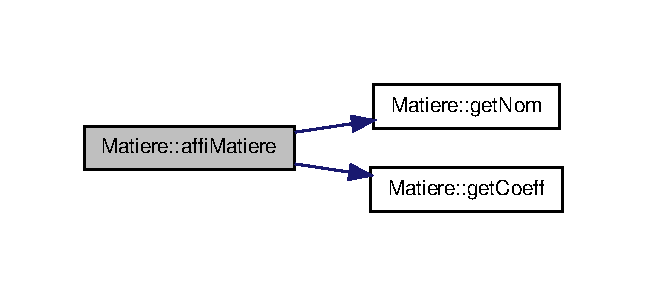
\includegraphics[width=310pt]{class_matiere_a40ce0a7003b3d771bbcb2c745a20ad1a_cgraph}
\end{center}
\end{figure}


\hypertarget{class_matiere_a3e50f81ac7893dbd989c9d06ff9af763}{\index{Matiere@{Matiere}!get\-Coeff@{get\-Coeff}}
\index{get\-Coeff@{get\-Coeff}!Matiere@{Matiere}}
\subsubsection[{get\-Coeff}]{\setlength{\rightskip}{0pt plus 5cm}int Matiere\-::get\-Coeff (
\begin{DoxyParamCaption}
{}
\end{DoxyParamCaption}
)}}\label{class_matiere_a3e50f81ac7893dbd989c9d06ff9af763}


$\ast$\-Permet de retourner le coeff de la matière 

\begin{DoxyReturn}{Renvoie}
le coeff de la matiere demander
\end{DoxyReturn}
Get the value of coeff \begin{DoxyReturn}{Renvoie}
the value of coeff 
\end{DoxyReturn}


Voici le graphe des appelants de cette fonction \-:
\nopagebreak
\begin{figure}[H]
\begin{center}
\leavevmode
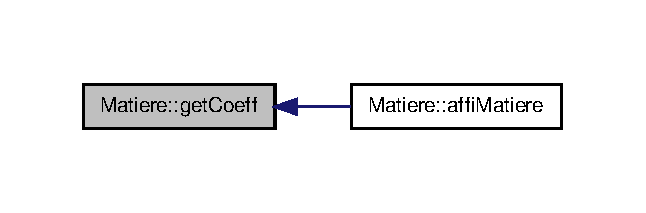
\includegraphics[width=310pt]{class_matiere_a3e50f81ac7893dbd989c9d06ff9af763_icgraph}
\end{center}
\end{figure}


\hypertarget{class_matiere_a103abd445b1bc378e0e3687875f4fcff}{\index{Matiere@{Matiere}!get\-Nom@{get\-Nom}}
\index{get\-Nom@{get\-Nom}!Matiere@{Matiere}}
\subsubsection[{get\-Nom}]{\setlength{\rightskip}{0pt plus 5cm}string Matiere\-::get\-Nom (
\begin{DoxyParamCaption}
{}
\end{DoxyParamCaption}
)}}\label{class_matiere_a103abd445b1bc378e0e3687875f4fcff}


$\ast$\-Permet de retourner le nom d'une matière 

\begin{DoxyReturn}{Renvoie}
le nom de la matière demander
\end{DoxyReturn}
Get the value of nom \begin{DoxyReturn}{Renvoie}
the value of nom 
\end{DoxyReturn}


Voici le graphe des appelants de cette fonction \-:
\nopagebreak
\begin{figure}[H]
\begin{center}
\leavevmode
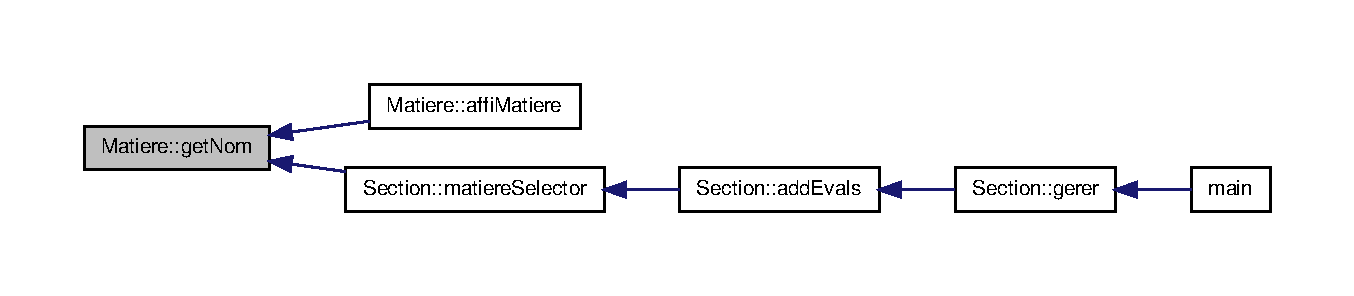
\includegraphics[width=350pt]{class_matiere_a103abd445b1bc378e0e3687875f4fcff_icgraph}
\end{center}
\end{figure}


\hypertarget{class_matiere_ac84968e1561a24e5118468edc2750f4f}{\index{Matiere@{Matiere}!saisie\-Matiere@{saisie\-Matiere}}
\index{saisie\-Matiere@{saisie\-Matiere}!Matiere@{Matiere}}
\subsubsection[{saisie\-Matiere}]{\setlength{\rightskip}{0pt plus 5cm}void Matiere\-::saisie\-Matiere (
\begin{DoxyParamCaption}
{}
\end{DoxyParamCaption}
)}}\label{class_matiere_ac84968e1561a24e5118468edc2750f4f}


saisir une Matière $\ast$\-Permet à l'utilisateur de saisir toutes les informations de la matière 



Voici le graphe d'appel pour cette fonction \-:
\nopagebreak
\begin{figure}[H]
\begin{center}
\leavevmode
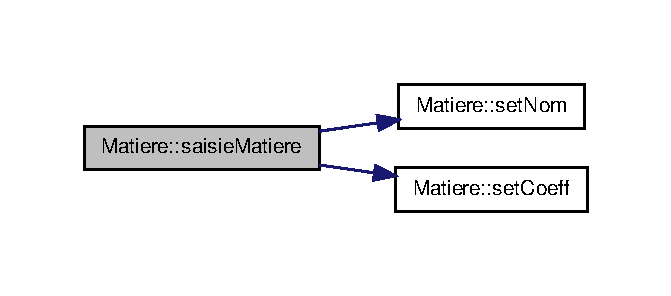
\includegraphics[width=322pt]{class_matiere_ac84968e1561a24e5118468edc2750f4f_cgraph}
\end{center}
\end{figure}




Voici le graphe des appelants de cette fonction \-:
\nopagebreak
\begin{figure}[H]
\begin{center}
\leavevmode
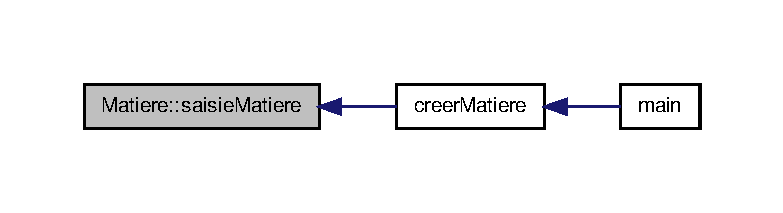
\includegraphics[width=350pt]{class_matiere_ac84968e1561a24e5118468edc2750f4f_icgraph}
\end{center}
\end{figure}


\hypertarget{class_matiere_aabf35dcc826eedca91490b8985d67da7}{\index{Matiere@{Matiere}!set\-Coeff@{set\-Coeff}}
\index{set\-Coeff@{set\-Coeff}!Matiere@{Matiere}}
\subsubsection[{set\-Coeff}]{\setlength{\rightskip}{0pt plus 5cm}void Matiere\-::set\-Coeff (
\begin{DoxyParamCaption}
\item[{int}]{new\-\_\-var}
\end{DoxyParamCaption}
)}}\label{class_matiere_aabf35dcc826eedca91490b8985d67da7}


$\ast$\-Permet de donner un coeff à une matière 

Set the value of coeff 
\begin{DoxyParams}{Paramètres}
{\em new\-\_\-var} & the new value of coeff \\
\hline
\end{DoxyParams}


Voici le graphe des appelants de cette fonction \-:
\nopagebreak
\begin{figure}[H]
\begin{center}
\leavevmode
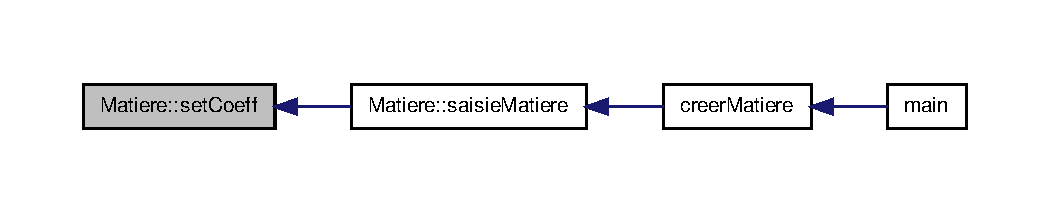
\includegraphics[width=350pt]{class_matiere_aabf35dcc826eedca91490b8985d67da7_icgraph}
\end{center}
\end{figure}


\hypertarget{class_matiere_ae0d9312f6cbddf446614ffa00d1750ae}{\index{Matiere@{Matiere}!set\-Nom@{set\-Nom}}
\index{set\-Nom@{set\-Nom}!Matiere@{Matiere}}
\subsubsection[{set\-Nom}]{\setlength{\rightskip}{0pt plus 5cm}void Matiere\-::set\-Nom (
\begin{DoxyParamCaption}
\item[{string}]{new\-\_\-var}
\end{DoxyParamCaption}
)}}\label{class_matiere_ae0d9312f6cbddf446614ffa00d1750ae}


$\ast$permet de donner un nom à une matière 

Set the value of nom 
\begin{DoxyParams}{Paramètres}
{\em new\-\_\-var} & the new value of nom \\
\hline
\end{DoxyParams}


Voici le graphe des appelants de cette fonction \-:
\nopagebreak
\begin{figure}[H]
\begin{center}
\leavevmode
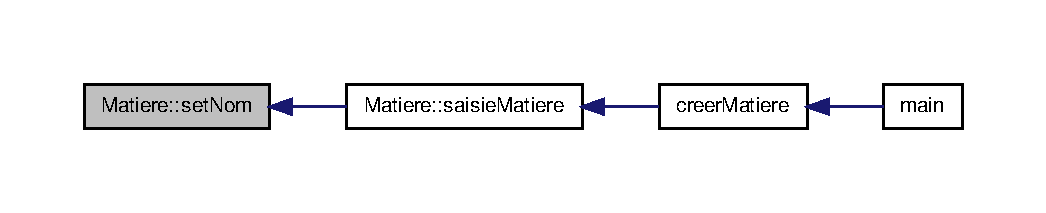
\includegraphics[width=350pt]{class_matiere_ae0d9312f6cbddf446614ffa00d1750ae_icgraph}
\end{center}
\end{figure}




La documentation de cette classe a été générée à partir des fichiers suivants \-:\begin{DoxyCompactItemize}
\item 
\hyperlink{_matiere_8h}{Matiere.\-h}\item 
\hyperlink{_matiere_8cpp}{Matiere.\-cpp}\end{DoxyCompactItemize}

\hypertarget{class_note}{\section{Référence de la classe Note}
\label{class_note}\index{Note@{Note}}
}


{\ttfamily \#include $<$Note.\-h$>$}



Graphe de collaboration de Note\-:
\nopagebreak
\begin{figure}[H]
\begin{center}
\leavevmode
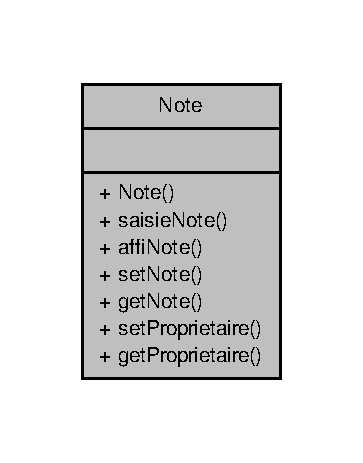
\includegraphics[width=174pt]{class_note__coll__graph}
\end{center}
\end{figure}
\subsection*{Fonctions membres publiques}
\begin{DoxyCompactItemize}
\item 
\hyperlink{class_note_a11dfaf68eb7a094b121add4adb18620e}{Note} ()
\item 
void \hyperlink{class_note_a50a10d0644153ef3be5f66c6b53634c2}{saisie\-Note} ()
\begin{DoxyCompactList}\small\item\em saisie d'une note $\ast$\-Permet de saisir les informations d'une note \end{DoxyCompactList}\item 
void \hyperlink{class_note_ac1f76f3565bdbc29c607dfbd8196d27e}{affi\-Note} ()
\begin{DoxyCompactList}\small\item\em affiche une note $\ast$\-Permet d'afficher les informations d'une note \end{DoxyCompactList}\item 
void \hyperlink{class_note_afc30ddbaca8f8ef44a2ccda7ffdd22d9}{set\-Note} (float new\-\_\-var)
\begin{DoxyCompactList}\small\item\em $\ast$\-Permet de donner une note \end{DoxyCompactList}\item 
float \hyperlink{class_note_a2360b36c3e33284e9d9d19331659c631}{get\-Note} ()
\begin{DoxyCompactList}\small\item\em $\ast$\-Permet de retourner la note \end{DoxyCompactList}\item 
void \hyperlink{class_note_aaae9bd761fbbdccfc70052f2d157afa4}{set\-Proprietaire} (\hyperlink{class_eleve}{Eleve} $\ast$new\-\_\-var)
\begin{DoxyCompactList}\small\item\em $\ast$\-Permet de donner un propriétaire à la note \end{DoxyCompactList}\item 
\hyperlink{class_eleve}{Eleve} $\ast$ \hyperlink{class_note_a986afc3571fe0035f727e8b90abda6e1}{get\-Proprietaire} ()
\begin{DoxyCompactList}\small\item\em $\ast$\-Permet de retourner le propriétaire de la note \end{DoxyCompactList}\end{DoxyCompactItemize}


\subsection{Description détaillée}
class \hyperlink{class_note}{Note} 

\subsection{Documentation des constructeurs et destructeur}
\hypertarget{class_note_a11dfaf68eb7a094b121add4adb18620e}{\index{Note@{Note}!Note@{Note}}
\index{Note@{Note}!Note@{Note}}
\subsubsection[{Note}]{\setlength{\rightskip}{0pt plus 5cm}Note\-::\-Note (
\begin{DoxyParamCaption}
{}
\end{DoxyParamCaption}
)}}\label{class_note_a11dfaf68eb7a094b121add4adb18620e}
Empty Constructor 

\subsection{Documentation des fonctions membres}
\hypertarget{class_note_ac1f76f3565bdbc29c607dfbd8196d27e}{\index{Note@{Note}!affi\-Note@{affi\-Note}}
\index{affi\-Note@{affi\-Note}!Note@{Note}}
\subsubsection[{affi\-Note}]{\setlength{\rightskip}{0pt plus 5cm}void Note\-::affi\-Note (
\begin{DoxyParamCaption}
{}
\end{DoxyParamCaption}
)}}\label{class_note_ac1f76f3565bdbc29c607dfbd8196d27e}


affiche une note $\ast$\-Permet d'afficher les informations d'une note 



Voici le graphe d'appel pour cette fonction \-:
\nopagebreak
\begin{figure}[H]
\begin{center}
\leavevmode
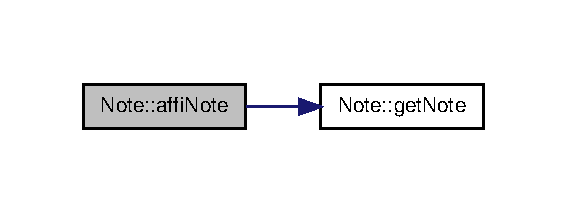
\includegraphics[width=272pt]{class_note_ac1f76f3565bdbc29c607dfbd8196d27e_cgraph}
\end{center}
\end{figure}


\hypertarget{class_note_a2360b36c3e33284e9d9d19331659c631}{\index{Note@{Note}!get\-Note@{get\-Note}}
\index{get\-Note@{get\-Note}!Note@{Note}}
\subsubsection[{get\-Note}]{\setlength{\rightskip}{0pt plus 5cm}float Note\-::get\-Note (
\begin{DoxyParamCaption}
{}
\end{DoxyParamCaption}
)}}\label{class_note_a2360b36c3e33284e9d9d19331659c631}


$\ast$\-Permet de retourner la note 

Get the value of note \begin{DoxyReturn}{Renvoie}
the value of note 
\end{DoxyReturn}


Voici le graphe des appelants de cette fonction \-:
\nopagebreak
\begin{figure}[H]
\begin{center}
\leavevmode
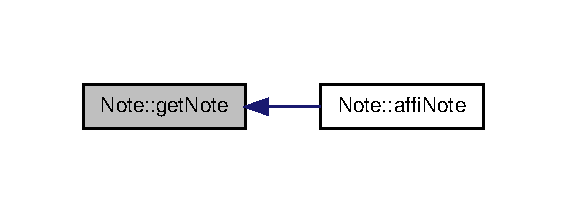
\includegraphics[width=272pt]{class_note_a2360b36c3e33284e9d9d19331659c631_icgraph}
\end{center}
\end{figure}


\hypertarget{class_note_a986afc3571fe0035f727e8b90abda6e1}{\index{Note@{Note}!get\-Proprietaire@{get\-Proprietaire}}
\index{get\-Proprietaire@{get\-Proprietaire}!Note@{Note}}
\subsubsection[{get\-Proprietaire}]{\setlength{\rightskip}{0pt plus 5cm}{\bf Eleve} $\ast$ Note\-::get\-Proprietaire (
\begin{DoxyParamCaption}
{}
\end{DoxyParamCaption}
)}}\label{class_note_a986afc3571fe0035f727e8b90abda6e1}


$\ast$\-Permet de retourner le propriétaire de la note 

Get the value of proprietaire \begin{DoxyReturn}{Renvoie}
the value of proprietaire 
\end{DoxyReturn}
\hypertarget{class_note_a50a10d0644153ef3be5f66c6b53634c2}{\index{Note@{Note}!saisie\-Note@{saisie\-Note}}
\index{saisie\-Note@{saisie\-Note}!Note@{Note}}
\subsubsection[{saisie\-Note}]{\setlength{\rightskip}{0pt plus 5cm}void Note\-::saisie\-Note (
\begin{DoxyParamCaption}
{}
\end{DoxyParamCaption}
)}}\label{class_note_a50a10d0644153ef3be5f66c6b53634c2}


saisie d'une note $\ast$\-Permet de saisir les informations d'une note 



Voici le graphe d'appel pour cette fonction \-:
\nopagebreak
\begin{figure}[H]
\begin{center}
\leavevmode
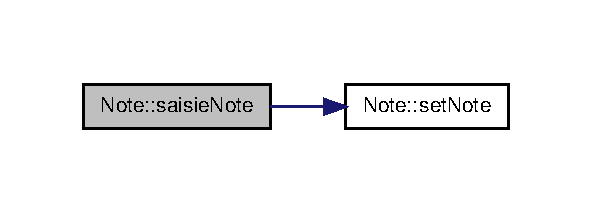
\includegraphics[width=284pt]{class_note_a50a10d0644153ef3be5f66c6b53634c2_cgraph}
\end{center}
\end{figure}




Voici le graphe des appelants de cette fonction \-:
\nopagebreak
\begin{figure}[H]
\begin{center}
\leavevmode
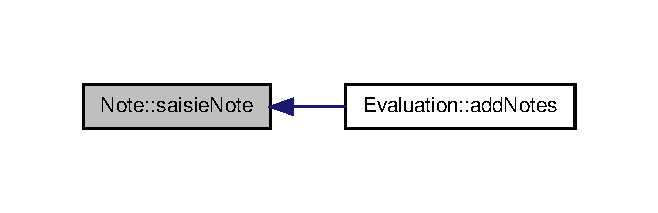
\includegraphics[width=316pt]{class_note_a50a10d0644153ef3be5f66c6b53634c2_icgraph}
\end{center}
\end{figure}


\hypertarget{class_note_afc30ddbaca8f8ef44a2ccda7ffdd22d9}{\index{Note@{Note}!set\-Note@{set\-Note}}
\index{set\-Note@{set\-Note}!Note@{Note}}
\subsubsection[{set\-Note}]{\setlength{\rightskip}{0pt plus 5cm}void Note\-::set\-Note (
\begin{DoxyParamCaption}
\item[{float}]{new\-\_\-var}
\end{DoxyParamCaption}
)}}\label{class_note_afc30ddbaca8f8ef44a2ccda7ffdd22d9}


$\ast$\-Permet de donner une note 

Set the value of note 
\begin{DoxyParams}{Paramètres}
{\em new\-\_\-var} & the new value of note \\
\hline
\end{DoxyParams}


Voici le graphe des appelants de cette fonction \-:
\nopagebreak
\begin{figure}[H]
\begin{center}
\leavevmode
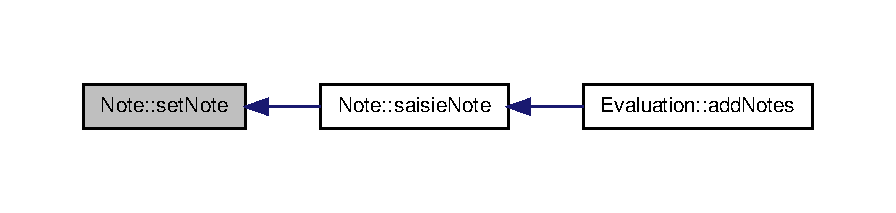
\includegraphics[width=350pt]{class_note_afc30ddbaca8f8ef44a2ccda7ffdd22d9_icgraph}
\end{center}
\end{figure}


\hypertarget{class_note_aaae9bd761fbbdccfc70052f2d157afa4}{\index{Note@{Note}!set\-Proprietaire@{set\-Proprietaire}}
\index{set\-Proprietaire@{set\-Proprietaire}!Note@{Note}}
\subsubsection[{set\-Proprietaire}]{\setlength{\rightskip}{0pt plus 5cm}void Note\-::set\-Proprietaire (
\begin{DoxyParamCaption}
\item[{{\bf Eleve} $\ast$}]{new\-\_\-var}
\end{DoxyParamCaption}
)}}\label{class_note_aaae9bd761fbbdccfc70052f2d157afa4}


$\ast$\-Permet de donner un propriétaire à la note 

Set the value of proprietaire 
\begin{DoxyParams}{Paramètres}
{\em new\-\_\-var} & the new value of proprietaire \\
\hline
\end{DoxyParams}


La documentation de cette classe a été générée à partir des fichiers suivants \-:\begin{DoxyCompactItemize}
\item 
\hyperlink{_note_8h}{Note.\-h}\item 
\hyperlink{_note_8cpp}{Note.\-cpp}\end{DoxyCompactItemize}

\hypertarget{class_section}{\section{Référence de la classe Section}
\label{class_section}\index{Section@{Section}}
}


{\ttfamily \#include $<$Section.\-h$>$}



Graphe de collaboration de Section\-:
\nopagebreak
\begin{figure}[H]
\begin{center}
\leavevmode
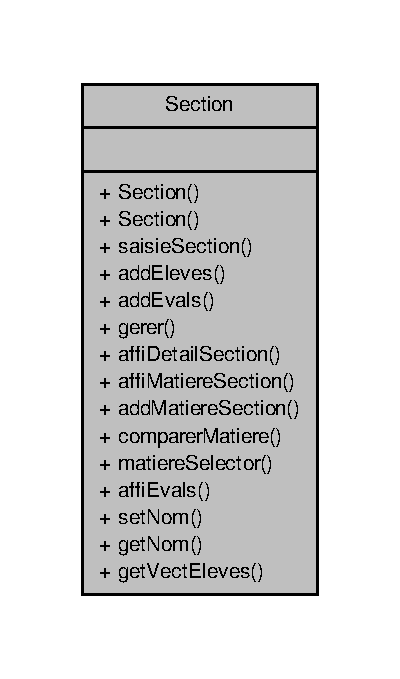
\includegraphics[width=192pt]{class_section__coll__graph}
\end{center}
\end{figure}
\subsection*{Fonctions membres publiques}
\begin{DoxyCompactItemize}
\item 
\hyperlink{class_section_a77b88e06692841ba49559d22a25a09f9}{Section} ()
\begin{DoxyCompactList}\small\item\em constructeur vide $\ast$\-Permet de créer une section sans donner de valeur au variable \end{DoxyCompactList}\item 
\hyperlink{class_section_aee5cac3104ae14544153dccfdc442b72}{Section} (string le\-Nom)
\begin{DoxyCompactList}\small\item\em constructeur nom $\ast$permet de créer une section en lui donnant le nom \end{DoxyCompactList}\item 
void \hyperlink{class_section_a7f3e53b28e0afcbba1c21168af9015bc}{saisie\-Section} ()
\begin{DoxyCompactList}\small\item\em saisir une section $\ast$\-Permet à l'utilisateur de saisir les valeurs d'une section \end{DoxyCompactList}\item 
void \hyperlink{class_section_abf60dc588ce5704e8cd259453cbe9e91}{add\-Eleves} ()
\begin{DoxyCompactList}\small\item\em ajouter élèves $\ast$\-Permet à l'utilisateur d'ajouter une élève dans la section \end{DoxyCompactList}\item 
void \hyperlink{class_section_a2009ece57cde4881da48efc6696ed691}{add\-Evals} ()
\begin{DoxyCompactList}\small\item\em ajouter évaluation $\ast$\-Permet à l'utilisateur d'ajouter une évaluation dans la section \end{DoxyCompactList}\item 
void \hyperlink{class_section_a59158781444f53654b89fad68291791b}{gerer} (vector$<$ \hyperlink{class_matiere}{Matiere} $>$ \hyperlink{main_8cpp_ac04b2ba8d7488df23bc7f9122d15434d}{vect\-Mat})
\begin{DoxyCompactList}\small\item\em menu section $\ast$\-Permet d'afficher le menu de la section et de gérer le choix de l'utilisateur \end{DoxyCompactList}\item 
void \hyperlink{class_section_a6279989607a517310651263aff2d42dd}{affi\-Detail\-Section} (vector$<$ \hyperlink{class_eleve}{Eleve} $>$ \&le\-Vecteur)
\begin{DoxyCompactList}\small\item\em afficher les détaille de la section $\ast$\-Permet d'afficher le nom de la section, le nom de tout les élèves et de toute les matière saisie dans celle-\/ci \end{DoxyCompactList}\item 
void \hyperlink{class_section_a0758af47447fe1099202b67e817c6cdb}{affi\-Matiere\-Section} (vector$<$ \hyperlink{class_matiere}{Matiere} $>$ \&le\-Vecteur)
\begin{DoxyCompactList}\small\item\em affiche les matières $\ast$\-Permet d'afficher toute les matières de la section \end{DoxyCompactList}\item 
void \hyperlink{class_section_a481421eaade6bf5935654a2386860eea}{add\-Matiere\-Section} (vector$<$ \hyperlink{class_matiere}{Matiere} $>$ \&le\-Vecteur)
\begin{DoxyCompactList}\small\item\em ajouter une matière à la section $\ast$\-Affiche les matières qui ne sont pas encore présente dans la section et l'utilisateur peut choisir celle qu'il veut ajouter à la section \end{DoxyCompactList}\item 
int \hyperlink{class_section_a6ab96944b37bfc813c3bac3c734951e9}{comparer\-Matiere} (string ma\-Matiere)
\begin{DoxyCompactList}\small\item\em comparer une matière $\ast$permet de comparer une matière du vecteur avec toute celle du vecteur qui contient les matière de la section \end{DoxyCompactList}\item 
\hyperlink{class_matiere}{Matiere} $\ast$ \hyperlink{class_section_a92511a0a21b91748cc244a2d220f76a5}{matiere\-Selector} (vector$<$ \hyperlink{class_matiere}{Matiere} $>$ \&le\-Vecteur)
\begin{DoxyCompactList}\small\item\em selection matière $\ast$\-Permet de d'afficher les matière et l'utilisateur peut sélectionner la matière qu'il veut \end{DoxyCompactList}\item 
void \hyperlink{class_section_a1b8aa93fa07ecafd30547ca0285738ae}{affi\-Evals} ()
\begin{DoxyCompactList}\small\item\em affiche évaluation $\ast$\-Permet d'afficher les évaluations \end{DoxyCompactList}\item 
void \hyperlink{class_section_a6d7313c0c0d9a1857db45f0b7978ebcc}{set\-Nom} (string new\-\_\-var)
\begin{DoxyCompactList}\small\item\em $\ast$\-Permet de donner un nom à la section \end{DoxyCompactList}\item 
string \hyperlink{class_section_a2f9835f8c6bfd5d3ae0eb53738fb51a7}{get\-Nom} ()
\begin{DoxyCompactList}\small\item\em $\ast$\-Permet de retourner le nom de la section \end{DoxyCompactList}\item 
vector$<$ \hyperlink{class_eleve}{Eleve} $>$ \hyperlink{class_section_aea3cca34d3659aba48926985bc279e42}{get\-Vect\-Eleves} ()
\begin{DoxyCompactList}\small\item\em $\ast$\-Permet de retourner le vecteur \end{DoxyCompactList}\end{DoxyCompactItemize}


\subsection{Description détaillée}
class \hyperlink{class_section}{Section} 

\subsection{Documentation des constructeurs et destructeur}
\hypertarget{class_section_a77b88e06692841ba49559d22a25a09f9}{\index{Section@{Section}!Section@{Section}}
\index{Section@{Section}!Section@{Section}}
\subsubsection[{Section}]{\setlength{\rightskip}{0pt plus 5cm}Section\-::\-Section (
\begin{DoxyParamCaption}
{}
\end{DoxyParamCaption}
)}}\label{class_section_a77b88e06692841ba49559d22a25a09f9}


constructeur vide $\ast$\-Permet de créer une section sans donner de valeur au variable 

\hypertarget{class_section_aee5cac3104ae14544153dccfdc442b72}{\index{Section@{Section}!Section@{Section}}
\index{Section@{Section}!Section@{Section}}
\subsubsection[{Section}]{\setlength{\rightskip}{0pt plus 5cm}Section\-::\-Section (
\begin{DoxyParamCaption}
\item[{string}]{le\-Nom}
\end{DoxyParamCaption}
)}}\label{class_section_aee5cac3104ae14544153dccfdc442b72}


constructeur nom $\ast$permet de créer une section en lui donnant le nom 



\subsection{Documentation des fonctions membres}
\hypertarget{class_section_abf60dc588ce5704e8cd259453cbe9e91}{\index{Section@{Section}!add\-Eleves@{add\-Eleves}}
\index{add\-Eleves@{add\-Eleves}!Section@{Section}}
\subsubsection[{add\-Eleves}]{\setlength{\rightskip}{0pt plus 5cm}void Section\-::add\-Eleves (
\begin{DoxyParamCaption}
{}
\end{DoxyParamCaption}
)}}\label{class_section_abf60dc588ce5704e8cd259453cbe9e91}


ajouter élèves $\ast$\-Permet à l'utilisateur d'ajouter une élève dans la section 



Voici le graphe d'appel pour cette fonction \-:
\nopagebreak
\begin{figure}[H]
\begin{center}
\leavevmode
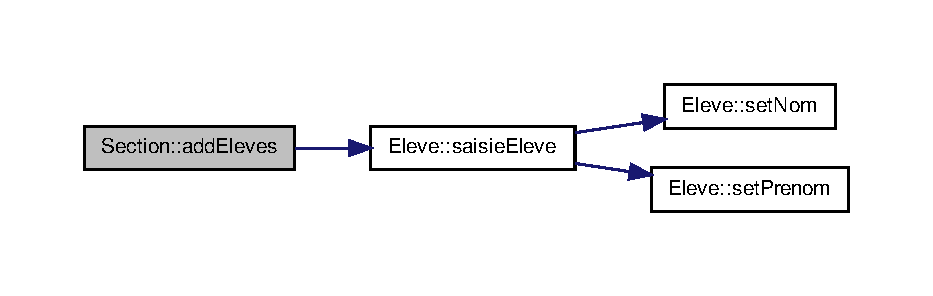
\includegraphics[width=350pt]{class_section_abf60dc588ce5704e8cd259453cbe9e91_cgraph}
\end{center}
\end{figure}




Voici le graphe des appelants de cette fonction \-:
\nopagebreak
\begin{figure}[H]
\begin{center}
\leavevmode
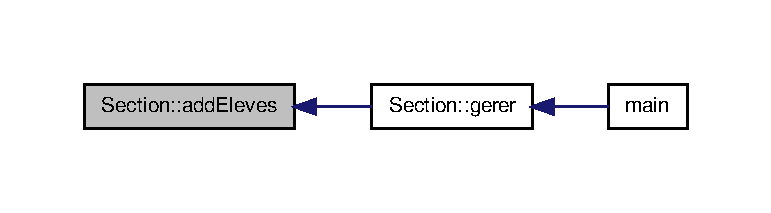
\includegraphics[width=350pt]{class_section_abf60dc588ce5704e8cd259453cbe9e91_icgraph}
\end{center}
\end{figure}


\hypertarget{class_section_a2009ece57cde4881da48efc6696ed691}{\index{Section@{Section}!add\-Evals@{add\-Evals}}
\index{add\-Evals@{add\-Evals}!Section@{Section}}
\subsubsection[{add\-Evals}]{\setlength{\rightskip}{0pt plus 5cm}void Section\-::add\-Evals (
\begin{DoxyParamCaption}
{}
\end{DoxyParamCaption}
)}}\label{class_section_a2009ece57cde4881da48efc6696ed691}


ajouter évaluation $\ast$\-Permet à l'utilisateur d'ajouter une évaluation dans la section 



Voici le graphe d'appel pour cette fonction \-:
\nopagebreak
\begin{figure}[H]
\begin{center}
\leavevmode
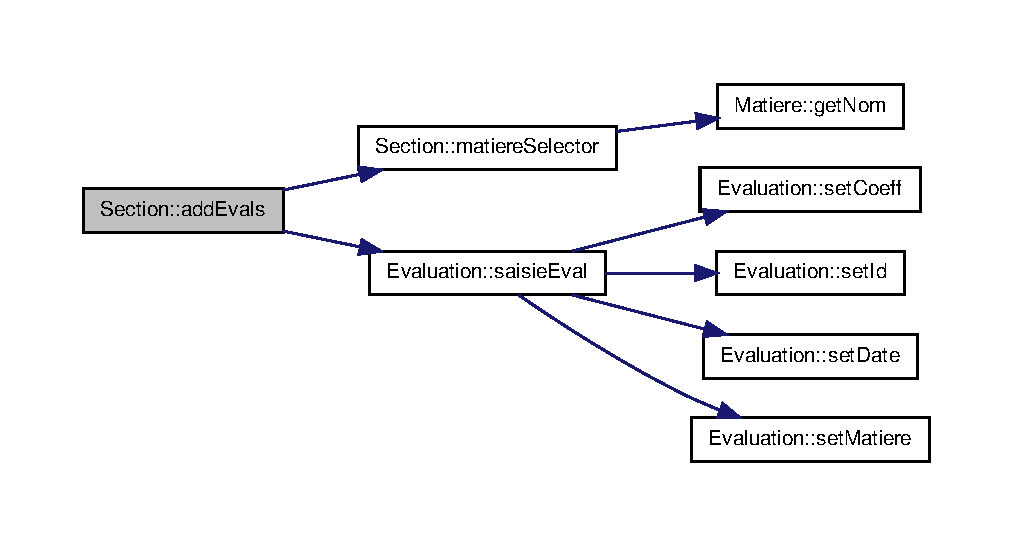
\includegraphics[width=350pt]{class_section_a2009ece57cde4881da48efc6696ed691_cgraph}
\end{center}
\end{figure}




Voici le graphe des appelants de cette fonction \-:
\nopagebreak
\begin{figure}[H]
\begin{center}
\leavevmode
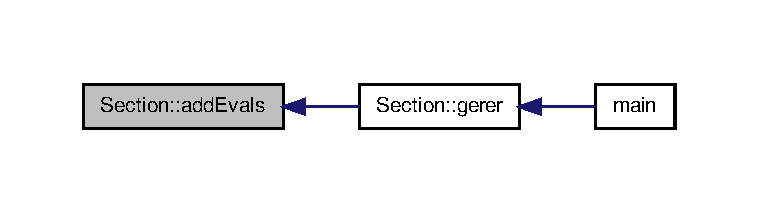
\includegraphics[width=350pt]{class_section_a2009ece57cde4881da48efc6696ed691_icgraph}
\end{center}
\end{figure}


\hypertarget{class_section_a481421eaade6bf5935654a2386860eea}{\index{Section@{Section}!add\-Matiere\-Section@{add\-Matiere\-Section}}
\index{add\-Matiere\-Section@{add\-Matiere\-Section}!Section@{Section}}
\subsubsection[{add\-Matiere\-Section}]{\setlength{\rightskip}{0pt plus 5cm}void Section\-::add\-Matiere\-Section (
\begin{DoxyParamCaption}
\item[{vector$<$ {\bf Matiere} $>$ \&}]{le\-Vecteur}
\end{DoxyParamCaption}
)}}\label{class_section_a481421eaade6bf5935654a2386860eea}


ajouter une matière à la section $\ast$\-Affiche les matières qui ne sont pas encore présente dans la section et l'utilisateur peut choisir celle qu'il veut ajouter à la section 


\begin{DoxyParams}{Paramètres}
{\em veceteur} & de toute les matières \\
\hline
\end{DoxyParams}


Voici le graphe d'appel pour cette fonction \-:
\nopagebreak
\begin{figure}[H]
\begin{center}
\leavevmode
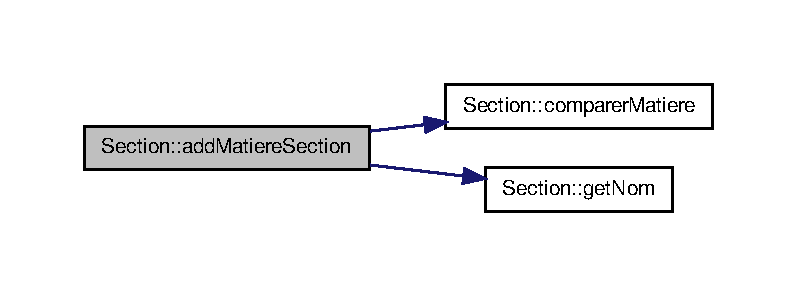
\includegraphics[width=350pt]{class_section_a481421eaade6bf5935654a2386860eea_cgraph}
\end{center}
\end{figure}




Voici le graphe des appelants de cette fonction \-:
\nopagebreak
\begin{figure}[H]
\begin{center}
\leavevmode
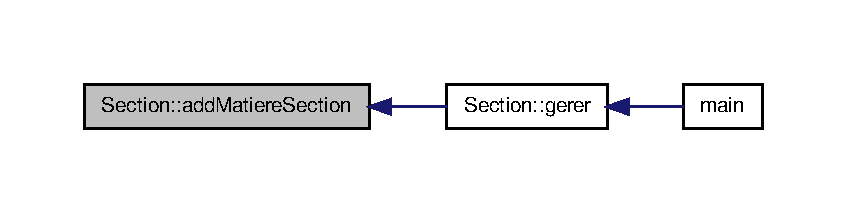
\includegraphics[width=350pt]{class_section_a481421eaade6bf5935654a2386860eea_icgraph}
\end{center}
\end{figure}


\hypertarget{class_section_a6279989607a517310651263aff2d42dd}{\index{Section@{Section}!affi\-Detail\-Section@{affi\-Detail\-Section}}
\index{affi\-Detail\-Section@{affi\-Detail\-Section}!Section@{Section}}
\subsubsection[{affi\-Detail\-Section}]{\setlength{\rightskip}{0pt plus 5cm}void Section\-::affi\-Detail\-Section (
\begin{DoxyParamCaption}
\item[{vector$<$ {\bf Eleve} $>$ \&}]{le\-Vecteur}
\end{DoxyParamCaption}
)}}\label{class_section_a6279989607a517310651263aff2d42dd}


afficher les détaille de la section $\ast$\-Permet d'afficher le nom de la section, le nom de tout les élèves et de toute les matière saisie dans celle-\/ci 



Voici le graphe d'appel pour cette fonction \-:
\nopagebreak
\begin{figure}[H]
\begin{center}
\leavevmode
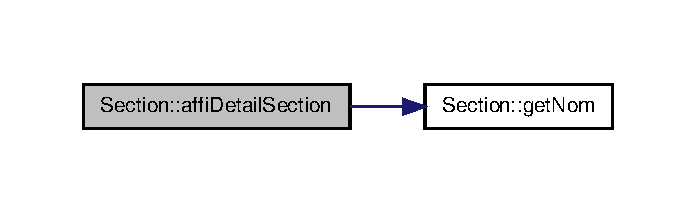
\includegraphics[width=334pt]{class_section_a6279989607a517310651263aff2d42dd_cgraph}
\end{center}
\end{figure}




Voici le graphe des appelants de cette fonction \-:
\nopagebreak
\begin{figure}[H]
\begin{center}
\leavevmode
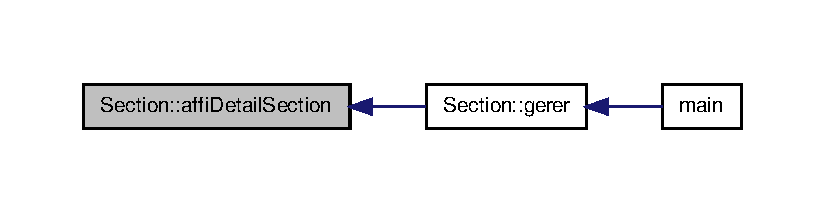
\includegraphics[width=350pt]{class_section_a6279989607a517310651263aff2d42dd_icgraph}
\end{center}
\end{figure}


\hypertarget{class_section_a1b8aa93fa07ecafd30547ca0285738ae}{\index{Section@{Section}!affi\-Evals@{affi\-Evals}}
\index{affi\-Evals@{affi\-Evals}!Section@{Section}}
\subsubsection[{affi\-Evals}]{\setlength{\rightskip}{0pt plus 5cm}void Section\-::affi\-Evals (
\begin{DoxyParamCaption}
{}
\end{DoxyParamCaption}
)}}\label{class_section_a1b8aa93fa07ecafd30547ca0285738ae}


affiche évaluation $\ast$\-Permet d'afficher les évaluations 



Voici le graphe des appelants de cette fonction \-:
\nopagebreak
\begin{figure}[H]
\begin{center}
\leavevmode
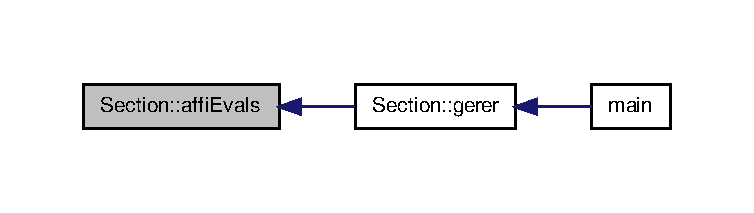
\includegraphics[width=350pt]{class_section_a1b8aa93fa07ecafd30547ca0285738ae_icgraph}
\end{center}
\end{figure}


\hypertarget{class_section_a0758af47447fe1099202b67e817c6cdb}{\index{Section@{Section}!affi\-Matiere\-Section@{affi\-Matiere\-Section}}
\index{affi\-Matiere\-Section@{affi\-Matiere\-Section}!Section@{Section}}
\subsubsection[{affi\-Matiere\-Section}]{\setlength{\rightskip}{0pt plus 5cm}void Section\-::affi\-Matiere\-Section (
\begin{DoxyParamCaption}
\item[{vector$<$ {\bf Matiere} $>$ \&}]{le\-Vecteur}
\end{DoxyParamCaption}
)}}\label{class_section_a0758af47447fe1099202b67e817c6cdb}


affiche les matières $\ast$\-Permet d'afficher toute les matières de la section 

\hypertarget{class_section_a6ab96944b37bfc813c3bac3c734951e9}{\index{Section@{Section}!comparer\-Matiere@{comparer\-Matiere}}
\index{comparer\-Matiere@{comparer\-Matiere}!Section@{Section}}
\subsubsection[{comparer\-Matiere}]{\setlength{\rightskip}{0pt plus 5cm}int Section\-::comparer\-Matiere (
\begin{DoxyParamCaption}
\item[{string}]{ma\-Matiere}
\end{DoxyParamCaption}
)}}\label{class_section_a6ab96944b37bfc813c3bac3c734951e9}


comparer une matière $\ast$permet de comparer une matière du vecteur avec toute celle du vecteur qui contient les matière de la section 


\begin{DoxyParams}{Paramètres}
{\em nom} & d'une matière \\
\hline
\end{DoxyParams}


Voici le graphe des appelants de cette fonction \-:
\nopagebreak
\begin{figure}[H]
\begin{center}
\leavevmode
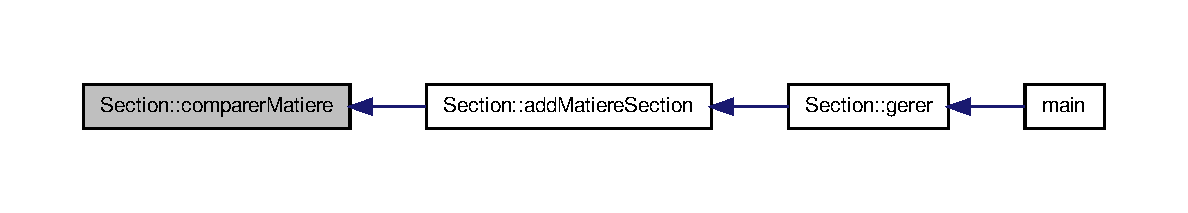
\includegraphics[width=350pt]{class_section_a6ab96944b37bfc813c3bac3c734951e9_icgraph}
\end{center}
\end{figure}


\hypertarget{class_section_a59158781444f53654b89fad68291791b}{\index{Section@{Section}!gerer@{gerer}}
\index{gerer@{gerer}!Section@{Section}}
\subsubsection[{gerer}]{\setlength{\rightskip}{0pt plus 5cm}void Section\-::gerer (
\begin{DoxyParamCaption}
\item[{vector$<$ {\bf Matiere} $>$}]{vect\-Mat}
\end{DoxyParamCaption}
)}}\label{class_section_a59158781444f53654b89fad68291791b}


menu section $\ast$\-Permet d'afficher le menu de la section et de gérer le choix de l'utilisateur 


\begin{DoxyParams}{Paramètres}
{\em vecteur} & de toute les matière éxistante \\
\hline
\end{DoxyParams}


Voici le graphe d'appel pour cette fonction \-:
\nopagebreak
\begin{figure}[H]
\begin{center}
\leavevmode
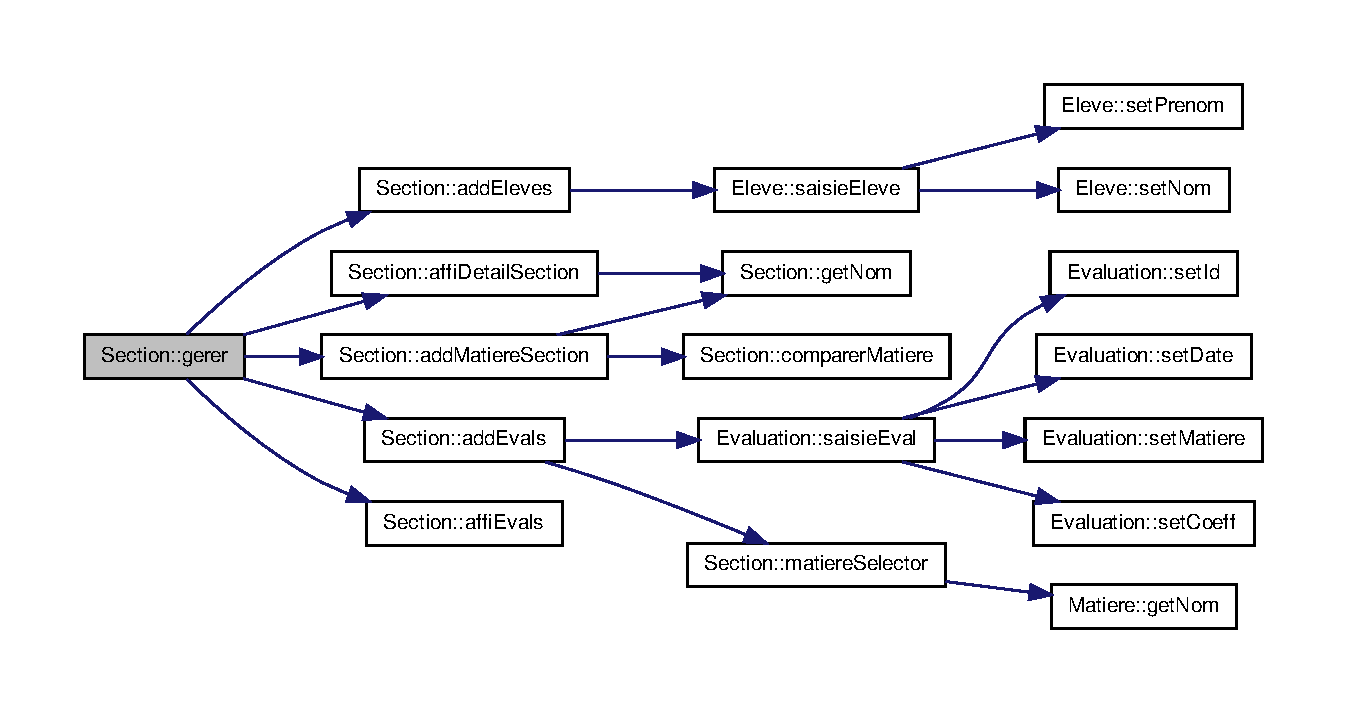
\includegraphics[width=350pt]{class_section_a59158781444f53654b89fad68291791b_cgraph}
\end{center}
\end{figure}




Voici le graphe des appelants de cette fonction \-:
\nopagebreak
\begin{figure}[H]
\begin{center}
\leavevmode
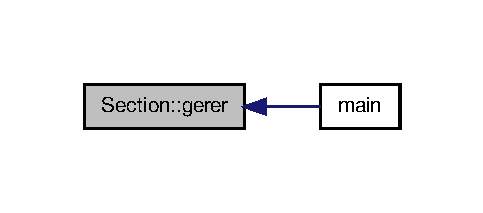
\includegraphics[width=232pt]{class_section_a59158781444f53654b89fad68291791b_icgraph}
\end{center}
\end{figure}


\hypertarget{class_section_a2f9835f8c6bfd5d3ae0eb53738fb51a7}{\index{Section@{Section}!get\-Nom@{get\-Nom}}
\index{get\-Nom@{get\-Nom}!Section@{Section}}
\subsubsection[{get\-Nom}]{\setlength{\rightskip}{0pt plus 5cm}string Section\-::get\-Nom (
\begin{DoxyParamCaption}
{}
\end{DoxyParamCaption}
)}}\label{class_section_a2f9835f8c6bfd5d3ae0eb53738fb51a7}


$\ast$\-Permet de retourner le nom de la section 

Get the value of nom \begin{DoxyReturn}{Renvoie}
the value of nom 
\end{DoxyReturn}


Voici le graphe des appelants de cette fonction \-:
\nopagebreak
\begin{figure}[H]
\begin{center}
\leavevmode
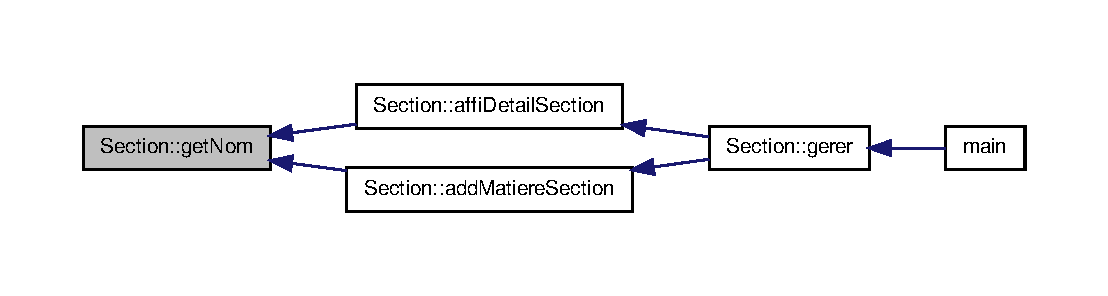
\includegraphics[width=350pt]{class_section_a2f9835f8c6bfd5d3ae0eb53738fb51a7_icgraph}
\end{center}
\end{figure}


\hypertarget{class_section_aea3cca34d3659aba48926985bc279e42}{\index{Section@{Section}!get\-Vect\-Eleves@{get\-Vect\-Eleves}}
\index{get\-Vect\-Eleves@{get\-Vect\-Eleves}!Section@{Section}}
\subsubsection[{get\-Vect\-Eleves}]{\setlength{\rightskip}{0pt plus 5cm}vector$<$ {\bf Eleve} $>$ Section\-::get\-Vect\-Eleves (
\begin{DoxyParamCaption}
{}
\end{DoxyParamCaption}
)}}\label{class_section_aea3cca34d3659aba48926985bc279e42}


$\ast$\-Permet de retourner le vecteur 

Get the value of vect\-Eleves \begin{DoxyReturn}{Renvoie}
the value of vect\-Eleves 
\end{DoxyReturn}
\hypertarget{class_section_a92511a0a21b91748cc244a2d220f76a5}{\index{Section@{Section}!matiere\-Selector@{matiere\-Selector}}
\index{matiere\-Selector@{matiere\-Selector}!Section@{Section}}
\subsubsection[{matiere\-Selector}]{\setlength{\rightskip}{0pt plus 5cm}{\bf Matiere} $\ast$ Section\-::matiere\-Selector (
\begin{DoxyParamCaption}
\item[{vector$<$ {\bf Matiere} $>$ \&}]{le\-Vecteur}
\end{DoxyParamCaption}
)}}\label{class_section_a92511a0a21b91748cc244a2d220f76a5}


selection matière $\ast$\-Permet de d'afficher les matière et l'utilisateur peut sélectionner la matière qu'il veut 



Voici le graphe d'appel pour cette fonction \-:
\nopagebreak
\begin{figure}[H]
\begin{center}
\leavevmode
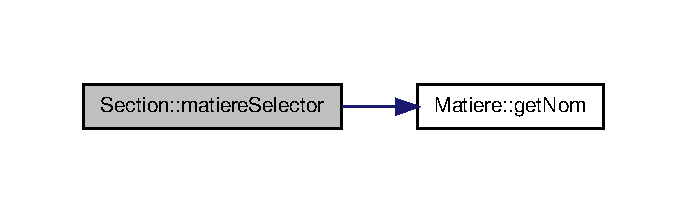
\includegraphics[width=330pt]{class_section_a92511a0a21b91748cc244a2d220f76a5_cgraph}
\end{center}
\end{figure}




Voici le graphe des appelants de cette fonction \-:
\nopagebreak
\begin{figure}[H]
\begin{center}
\leavevmode
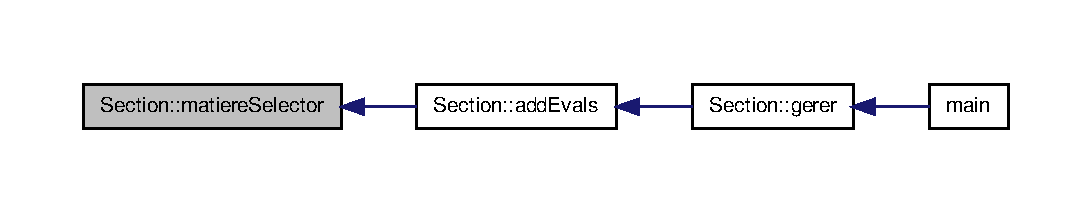
\includegraphics[width=350pt]{class_section_a92511a0a21b91748cc244a2d220f76a5_icgraph}
\end{center}
\end{figure}


\hypertarget{class_section_a7f3e53b28e0afcbba1c21168af9015bc}{\index{Section@{Section}!saisie\-Section@{saisie\-Section}}
\index{saisie\-Section@{saisie\-Section}!Section@{Section}}
\subsubsection[{saisie\-Section}]{\setlength{\rightskip}{0pt plus 5cm}void Section\-::saisie\-Section (
\begin{DoxyParamCaption}
{}
\end{DoxyParamCaption}
)}}\label{class_section_a7f3e53b28e0afcbba1c21168af9015bc}


saisir une section $\ast$\-Permet à l'utilisateur de saisir les valeurs d'une section 



Voici le graphe d'appel pour cette fonction \-:
\nopagebreak
\begin{figure}[H]
\begin{center}
\leavevmode
\includegraphics[width=320pt]{class_section_a7f3e53b28e0afcbba1c21168af9015bc_cgraph}
\end{center}
\end{figure}




Voici le graphe des appelants de cette fonction \-:
\nopagebreak
\begin{figure}[H]
\begin{center}
\leavevmode
\includegraphics[width=350pt]{class_section_a7f3e53b28e0afcbba1c21168af9015bc_icgraph}
\end{center}
\end{figure}


\hypertarget{class_section_a6d7313c0c0d9a1857db45f0b7978ebcc}{\index{Section@{Section}!set\-Nom@{set\-Nom}}
\index{set\-Nom@{set\-Nom}!Section@{Section}}
\subsubsection[{set\-Nom}]{\setlength{\rightskip}{0pt plus 5cm}void Section\-::set\-Nom (
\begin{DoxyParamCaption}
\item[{string}]{new\-\_\-var}
\end{DoxyParamCaption}
)}}\label{class_section_a6d7313c0c0d9a1857db45f0b7978ebcc}


$\ast$\-Permet de donner un nom à la section 

Set the value of nom 
\begin{DoxyParams}{Paramètres}
{\em new\-\_\-var} & the new value of nom \\
\hline
\end{DoxyParams}


Voici le graphe des appelants de cette fonction \-:
\nopagebreak
\begin{figure}[H]
\begin{center}
\leavevmode
\includegraphics[width=350pt]{class_section_a6d7313c0c0d9a1857db45f0b7978ebcc_icgraph}
\end{center}
\end{figure}




La documentation de cette classe a été générée à partir des fichiers suivants \-:\begin{DoxyCompactItemize}
\item 
\hyperlink{_section_8h}{Section.\-h}\item 
\hyperlink{_section_8cpp}{Section.\-cpp}\end{DoxyCompactItemize}

\chapter{Documentation des fichiers}
\hypertarget{eleve_8cpp}{\section{Référence du fichier eleve.\-cpp}
\label{eleve_8cpp}\index{eleve.\-cpp@{eleve.\-cpp}}
}
{\ttfamily \#include \char`\"{}eleve.\-h\char`\"{}}\\*
Graphe des dépendances par inclusion de eleve.\-cpp\-:
\nopagebreak
\begin{figure}[H]
\begin{center}
\leavevmode
\includegraphics[width=192pt]{eleve_8cpp__incl}
\end{center}
\end{figure}

\hypertarget{eleve_8h}{\section{Référence du fichier eleve.\-h}
\label{eleve_8h}\index{eleve.\-h@{eleve.\-h}}
}
{\ttfamily \#include $<$iostream$>$}\\*
{\ttfamily \#include $<$string$>$}\\*
Graphe des dépendances par inclusion de eleve.\-h\-:
\nopagebreak
\begin{figure}[H]
\begin{center}
\leavevmode
\includegraphics[width=192pt]{eleve_8h__incl}
\end{center}
\end{figure}
Ce graphe montre quels fichiers incluent directement ou indirectement ce fichier \-:
\nopagebreak
\begin{figure}[H]
\begin{center}
\leavevmode
\includegraphics[width=350pt]{eleve_8h__dep__incl}
\end{center}
\end{figure}
\subsection*{Classes}
\begin{DoxyCompactItemize}
\item 
class \hyperlink{class_eleve}{Eleve}
\end{DoxyCompactItemize}

\hypertarget{_evaluation_8cpp}{\section{Référence du fichier Evaluation.\-cpp}
\label{_evaluation_8cpp}\index{Evaluation.\-cpp@{Evaluation.\-cpp}}
}
{\ttfamily \#include \char`\"{}Evaluation.\-h\char`\"{}}\\*
Graphe des dépendances par inclusion de Evaluation.\-cpp\-:
\nopagebreak
\begin{figure}[H]
\begin{center}
\leavevmode
\includegraphics[width=350pt]{_evaluation_8cpp__incl}
\end{center}
\end{figure}

\hypertarget{_evaluation_8h}{\section{Référence du fichier Evaluation.\-h}
\label{_evaluation_8h}\index{Evaluation.\-h@{Evaluation.\-h}}
}
{\ttfamily \#include \char`\"{}Matiere.\-h\char`\"{}}\\*
{\ttfamily \#include \char`\"{}Note.\-h\char`\"{}}\\*
{\ttfamily \#include $<$string$>$}\\*
{\ttfamily \#include $<$vector$>$}\\*
{\ttfamily \#include $<$iostream$>$}\\*
Graphe des dépendances par inclusion de Evaluation.\-h\-:
\nopagebreak
\begin{figure}[H]
\begin{center}
\leavevmode
\includegraphics[width=350pt]{_evaluation_8h__incl}
\end{center}
\end{figure}
Ce graphe montre quels fichiers incluent directement ou indirectement ce fichier \-:
\nopagebreak
\begin{figure}[H]
\begin{center}
\leavevmode
\includegraphics[width=281pt]{_evaluation_8h__dep__incl}
\end{center}
\end{figure}
\subsection*{Classes}
\begin{DoxyCompactItemize}
\item 
class \hyperlink{class_evaluation}{Evaluation}
\end{DoxyCompactItemize}

\hypertarget{main_8cpp}{\section{Référence du fichier main.\-cpp}
\label{main_8cpp}\index{main.\-cpp@{main.\-cpp}}
}
{\ttfamily \#include $<$iostream$>$}\\*
{\ttfamily \#include $<$vector$>$}\\*
{\ttfamily \#include \char`\"{}eleve.\-h\char`\"{}}\\*
{\ttfamily \#include \char`\"{}Section.\-h\char`\"{}}\\*
{\ttfamily \#include \char`\"{}Matiere.\-h\char`\"{}}\\*
{\ttfamily \#include \char`\"{}Note.\-h\char`\"{}}\\*
Graphe des dépendances par inclusion de main.\-cpp\-:
\nopagebreak
\begin{figure}[H]
\begin{center}
\leavevmode
\includegraphics[width=350pt]{main_8cpp__incl}
\end{center}
\end{figure}
\subsection*{Fonctions}
\begin{DoxyCompactItemize}
\item 
void \hyperlink{main_8cpp_a060b1b9a54b301c0ef6718410c616044}{creer\-Section} ()
\item 
void \hyperlink{main_8cpp_a5074e8571076bbfa1bc2a053297520b7}{affi\-Section} (vector$<$ \hyperlink{class_section}{Section} $>$ \&le\-Vecteur)
\item 
\hyperlink{class_section}{Section} $\ast$ \hyperlink{main_8cpp_ab4da989a5a85c62e58b2aaaa560d541c}{section\-Selector} (vector$<$ \hyperlink{class_section}{Section} $>$ \&le\-Vecteur)
\item 
void \hyperlink{main_8cpp_a55645d67bf6c29003ffa1ac4af8327e7}{affi\-Matiere} (vector$<$ \hyperlink{class_matiere}{Matiere} $>$ \&le\-Vecteur)
\item 
void \hyperlink{main_8cpp_a0e3712f2940cab09560fc250f16e63cc}{creer\-Matiere} ()
\item 
int \hyperlink{main_8cpp_ae66f6b31b5ad750f1fe042a706a4e3d4}{main} ()
\end{DoxyCompactItemize}
\subsection*{Variables}
\begin{DoxyCompactItemize}
\item 
vector$<$ \hyperlink{class_section}{Section} $>$ \hyperlink{main_8cpp_a4ccab3cf64964dcae416ebcbfe34b49a}{vect\-Sec}
\item 
vector$<$ \hyperlink{class_matiere}{Matiere} $>$ \hyperlink{main_8cpp_ac04b2ba8d7488df23bc7f9122d15434d}{vect\-Mat}
\end{DoxyCompactItemize}


\subsection{Documentation des fonctions}
\hypertarget{main_8cpp_a55645d67bf6c29003ffa1ac4af8327e7}{\index{main.\-cpp@{main.\-cpp}!affi\-Matiere@{affi\-Matiere}}
\index{affi\-Matiere@{affi\-Matiere}!main.cpp@{main.\-cpp}}
\subsubsection[{affi\-Matiere}]{\setlength{\rightskip}{0pt plus 5cm}void affi\-Matiere (
\begin{DoxyParamCaption}
\item[{vector$<$ {\bf Matiere} $>$ \&}]{le\-Vecteur}
\end{DoxyParamCaption}
)}}\label{main_8cpp_a55645d67bf6c29003ffa1ac4af8327e7}


Voici le graphe des appelants de cette fonction \-:
\nopagebreak
\begin{figure}[H]
\begin{center}
\leavevmode
\includegraphics[width=216pt]{main_8cpp_a55645d67bf6c29003ffa1ac4af8327e7_icgraph}
\end{center}
\end{figure}


\hypertarget{main_8cpp_a5074e8571076bbfa1bc2a053297520b7}{\index{main.\-cpp@{main.\-cpp}!affi\-Section@{affi\-Section}}
\index{affi\-Section@{affi\-Section}!main.cpp@{main.\-cpp}}
\subsubsection[{affi\-Section}]{\setlength{\rightskip}{0pt plus 5cm}void affi\-Section (
\begin{DoxyParamCaption}
\item[{vector$<$ {\bf Section} $>$ \&}]{le\-Vecteur}
\end{DoxyParamCaption}
)}}\label{main_8cpp_a5074e8571076bbfa1bc2a053297520b7}


Voici le graphe des appelants de cette fonction \-:
\nopagebreak
\begin{figure}[H]
\begin{center}
\leavevmode
\includegraphics[width=338pt]{main_8cpp_a5074e8571076bbfa1bc2a053297520b7_icgraph}
\end{center}
\end{figure}


\hypertarget{main_8cpp_a0e3712f2940cab09560fc250f16e63cc}{\index{main.\-cpp@{main.\-cpp}!creer\-Matiere@{creer\-Matiere}}
\index{creer\-Matiere@{creer\-Matiere}!main.cpp@{main.\-cpp}}
\subsubsection[{creer\-Matiere}]{\setlength{\rightskip}{0pt plus 5cm}void creer\-Matiere (
\begin{DoxyParamCaption}
{}
\end{DoxyParamCaption}
)}}\label{main_8cpp_a0e3712f2940cab09560fc250f16e63cc}


Voici le graphe d'appel pour cette fonction \-:
\nopagebreak
\begin{figure}[H]
\begin{center}
\leavevmode
\includegraphics[width=350pt]{main_8cpp_a0e3712f2940cab09560fc250f16e63cc_cgraph}
\end{center}
\end{figure}




Voici le graphe des appelants de cette fonction \-:
\nopagebreak
\begin{figure}[H]
\begin{center}
\leavevmode
\includegraphics[width=226pt]{main_8cpp_a0e3712f2940cab09560fc250f16e63cc_icgraph}
\end{center}
\end{figure}


\hypertarget{main_8cpp_a060b1b9a54b301c0ef6718410c616044}{\index{main.\-cpp@{main.\-cpp}!creer\-Section@{creer\-Section}}
\index{creer\-Section@{creer\-Section}!main.cpp@{main.\-cpp}}
\subsubsection[{creer\-Section}]{\setlength{\rightskip}{0pt plus 5cm}void creer\-Section (
\begin{DoxyParamCaption}
{}
\end{DoxyParamCaption}
)}}\label{main_8cpp_a060b1b9a54b301c0ef6718410c616044}


Voici le graphe d'appel pour cette fonction \-:
\nopagebreak
\begin{figure}[H]
\begin{center}
\leavevmode
\includegraphics[width=350pt]{main_8cpp_a060b1b9a54b301c0ef6718410c616044_cgraph}
\end{center}
\end{figure}




Voici le graphe des appelants de cette fonction \-:
\nopagebreak
\begin{figure}[H]
\begin{center}
\leavevmode
\includegraphics[width=226pt]{main_8cpp_a060b1b9a54b301c0ef6718410c616044_icgraph}
\end{center}
\end{figure}


\hypertarget{main_8cpp_ae66f6b31b5ad750f1fe042a706a4e3d4}{\index{main.\-cpp@{main.\-cpp}!main@{main}}
\index{main@{main}!main.cpp@{main.\-cpp}}
\subsubsection[{main}]{\setlength{\rightskip}{0pt plus 5cm}int main (
\begin{DoxyParamCaption}
{}
\end{DoxyParamCaption}
)}}\label{main_8cpp_ae66f6b31b5ad750f1fe042a706a4e3d4}


Voici le graphe d'appel pour cette fonction \-:
\nopagebreak
\begin{figure}[H]
\begin{center}
\leavevmode
\includegraphics[width=350pt]{main_8cpp_ae66f6b31b5ad750f1fe042a706a4e3d4_cgraph}
\end{center}
\end{figure}


\hypertarget{main_8cpp_ab4da989a5a85c62e58b2aaaa560d541c}{\index{main.\-cpp@{main.\-cpp}!section\-Selector@{section\-Selector}}
\index{section\-Selector@{section\-Selector}!main.cpp@{main.\-cpp}}
\subsubsection[{section\-Selector}]{\setlength{\rightskip}{0pt plus 5cm}{\bf Section}$\ast$ section\-Selector (
\begin{DoxyParamCaption}
\item[{vector$<$ {\bf Section} $>$ \&}]{le\-Vecteur}
\end{DoxyParamCaption}
)}}\label{main_8cpp_ab4da989a5a85c62e58b2aaaa560d541c}


Voici le graphe d'appel pour cette fonction \-:
\nopagebreak
\begin{figure}[H]
\begin{center}
\leavevmode
\includegraphics[width=264pt]{main_8cpp_ab4da989a5a85c62e58b2aaaa560d541c_cgraph}
\end{center}
\end{figure}




Voici le graphe des appelants de cette fonction \-:
\nopagebreak
\begin{figure}[H]
\begin{center}
\leavevmode
\includegraphics[width=238pt]{main_8cpp_ab4da989a5a85c62e58b2aaaa560d541c_icgraph}
\end{center}
\end{figure}




\subsection{Documentation des variables}
\hypertarget{main_8cpp_ac04b2ba8d7488df23bc7f9122d15434d}{\index{main.\-cpp@{main.\-cpp}!vect\-Mat@{vect\-Mat}}
\index{vect\-Mat@{vect\-Mat}!main.cpp@{main.\-cpp}}
\subsubsection[{vect\-Mat}]{\setlength{\rightskip}{0pt plus 5cm}vector$<${\bf Matiere}$>$ vect\-Mat}}\label{main_8cpp_ac04b2ba8d7488df23bc7f9122d15434d}
\hypertarget{main_8cpp_a4ccab3cf64964dcae416ebcbfe34b49a}{\index{main.\-cpp@{main.\-cpp}!vect\-Sec@{vect\-Sec}}
\index{vect\-Sec@{vect\-Sec}!main.cpp@{main.\-cpp}}
\subsubsection[{vect\-Sec}]{\setlength{\rightskip}{0pt plus 5cm}vector$<${\bf Section}$>$ vect\-Sec}}\label{main_8cpp_a4ccab3cf64964dcae416ebcbfe34b49a}

\hypertarget{_matiere_8cpp}{\section{Référence du fichier Matiere.\-cpp}
\label{_matiere_8cpp}\index{Matiere.\-cpp@{Matiere.\-cpp}}
}
{\ttfamily \#include \char`\"{}Matiere.\-h\char`\"{}}\\*
Graphe des dépendances par inclusion de Matiere.\-cpp\-:
\nopagebreak
\begin{figure}[H]
\begin{center}
\leavevmode
\includegraphics[width=192pt]{_matiere_8cpp__incl}
\end{center}
\end{figure}

\hypertarget{_matiere_8h}{\section{Référence du fichier Matiere.\-h}
\label{_matiere_8h}\index{Matiere.\-h@{Matiere.\-h}}
}
{\ttfamily \#include $<$iostream$>$}\\*
{\ttfamily \#include $<$string$>$}\\*
Graphe des dépendances par inclusion de Matiere.\-h\-:
\nopagebreak
\begin{figure}[H]
\begin{center}
\leavevmode
\includegraphics[width=192pt]{_matiere_8h__incl}
\end{center}
\end{figure}
Ce graphe montre quels fichiers incluent directement ou indirectement ce fichier \-:
\nopagebreak
\begin{figure}[H]
\begin{center}
\leavevmode
\includegraphics[width=350pt]{_matiere_8h__dep__incl}
\end{center}
\end{figure}
\subsection*{Classes}
\begin{DoxyCompactItemize}
\item 
class \hyperlink{class_matiere}{Matiere}
\end{DoxyCompactItemize}

\hypertarget{_note_8cpp}{\section{Référence du fichier Note.\-cpp}
\label{_note_8cpp}\index{Note.\-cpp@{Note.\-cpp}}
}
{\ttfamily \#include \char`\"{}Note.\-h\char`\"{}}\\*
Graphe des dépendances par inclusion de Note.\-cpp\-:
\nopagebreak
\begin{figure}[H]
\begin{center}
\leavevmode
\includegraphics[width=211pt]{_note_8cpp__incl}
\end{center}
\end{figure}

\hypertarget{_note_8h}{\section{Référence du fichier Note.\-h}
\label{_note_8h}\index{Note.\-h@{Note.\-h}}
}
{\ttfamily \#include \char`\"{}eleve.\-h\char`\"{}}\\*
{\ttfamily \#include $<$string$>$}\\*
{\ttfamily \#include $<$iostream$>$}\\*
Graphe des dépendances par inclusion de Note.\-h\-:
\nopagebreak
\begin{figure}[H]
\begin{center}
\leavevmode
\includegraphics[width=211pt]{_note_8h__incl}
\end{center}
\end{figure}
Ce graphe montre quels fichiers incluent directement ou indirectement ce fichier \-:
\nopagebreak
\begin{figure}[H]
\begin{center}
\leavevmode
\includegraphics[width=350pt]{_note_8h__dep__incl}
\end{center}
\end{figure}
\subsection*{Classes}
\begin{DoxyCompactItemize}
\item 
class \hyperlink{class_note}{Note}
\end{DoxyCompactItemize}

\hypertarget{_section_8cpp}{\section{Référence du fichier Section.\-cpp}
\label{_section_8cpp}\index{Section.\-cpp@{Section.\-cpp}}
}
{\ttfamily \#include \char`\"{}Section.\-h\char`\"{}}\\*
Graphe des dépendances par inclusion de Section.\-cpp\-:
\nopagebreak
\begin{figure}[H]
\begin{center}
\leavevmode
\includegraphics[width=350pt]{_section_8cpp__incl}
\end{center}
\end{figure}

\hypertarget{_section_8h}{\section{Référence du fichier Section.\-h}
\label{_section_8h}\index{Section.\-h@{Section.\-h}}
}
{\ttfamily \#include \char`\"{}eleve.\-h\char`\"{}}\\*
{\ttfamily \#include \char`\"{}Evaluation.\-h\char`\"{}}\\*
{\ttfamily \#include $<$string$>$}\\*
{\ttfamily \#include $<$vector$>$}\\*
{\ttfamily \#include $<$iostream$>$}\\*
Graphe des dépendances par inclusion de Section.\-h\-:
\nopagebreak
\begin{figure}[H]
\begin{center}
\leavevmode
\includegraphics[width=350pt]{_section_8h__incl}
\end{center}
\end{figure}
Ce graphe montre quels fichiers incluent directement ou indirectement ce fichier \-:
\nopagebreak
\begin{figure}[H]
\begin{center}
\leavevmode
\includegraphics[width=222pt]{_section_8h__dep__incl}
\end{center}
\end{figure}
\subsection*{Classes}
\begin{DoxyCompactItemize}
\item 
class \hyperlink{class_section}{Section}
\end{DoxyCompactItemize}

\printindex
\end{document}
